%%%%%%%%%%%%%%%%%%%%%%%%%%%%%%%%%%%
%This is the LaTeX ARTICLE template for RSC journals
%Copyright The Royal Society of Chemistry 2016
%%%%%%%%%%%%%%%%%%%%%%%%%%%%%%%%%%%

\documentclass[twoside,twocolumn,9pt]{article}

\usepackage{tgheros}
\renewcommand{\familydefault}{\sfdefault}

\usepackage{extsizes}
\usepackage[super,sort&compress,comma]{natbib} 
\usepackage[version=3]{mhchem}
\usepackage[left=1.5cm, right=1.5cm, top=1.785cm, bottom=2.0cm]{geometry}
\usepackage{balance}
\usepackage{mathptmx}
\usepackage{sectsty}
\usepackage{graphicx} 
\usepackage{lastpage}
\usepackage[format=plain,justification=justified,singlelinecheck=false,font={stretch=1.125,small,sf},labelfont=bf,labelsep=space]{caption}
\usepackage{float}
\usepackage{fancyhdr}
\usepackage{fnpos}
\usepackage[english]{babel}
\addto{\captionsenglish}{%
  \renewcommand{\refname}{Notes and references}
}
\usepackage{array}
\usepackage{droidsans}
\usepackage{charter}
\usepackage[T1]{fontenc}
\usepackage[usenames,dvipsnames]{xcolor}
\usepackage{setspace}
\usepackage[compact]{titlesec}
\usepackage[utf8]{inputenc}
\usepackage{physics}
\usepackage{tikz}
\usetikzlibrary{shapes.geometric}

\usepackage[mathscr]{euscript}  % \mathscr

%%%Please don't disable any packages in the preamble, as this may cause the template to display incorrectly.%%%


\usepackage{xcolor}
\definecolor{ugent_blue}{RGB}{30, 100, 200}
\definecolor{ugent_yellow}{cmyk}{.0, .10, 1, 0}

\usepackage{titlesec}
\titleformat{\section}
{\color{ugent_blue}\normalfont\Large\bfseries}
{\color{ugent_blue}\thesection}{1em}{}

\usepackage[colorlinks=true,linkcolor=black,citecolor=ugent_blue]{hyperref}
\usepackage{cleveref}

\usepackage{lineno}
\linenumbers

%\AtEveryCite{\color{ugent_blue}}




\usepackage{epstopdf}%This line makes .eps figures into .pdf - please comment out if not required.

\definecolor{cream}{RGB}{222,217,201}

\begin{document}

\pagestyle{fancy}
\thispagestyle{plain}
\fancypagestyle{plain}{
%%%HEADER%%%
\renewcommand{\headrulewidth}{0pt}
}
%%%END OF HEADER%%%

%%%PAGE SETUP - Please do not change any commands within this section%%%
\makeFNbottom
\makeatletter
\renewcommand\LARGE{\@setfontsize\LARGE{15pt}{17}}
\renewcommand\Large{\@setfontsize\Large{12pt}{14}}
\renewcommand\large{\@setfontsize\large{10pt}{12}}
\renewcommand\footnotesize{\@setfontsize\footnotesize{7pt}{10}}
\makeatother

\renewcommand{\thefootnote}{\fnsymbol{footnote}}
\renewcommand\footnoterule{\vspace*{1pt}% 
\color{cream}\hrule width 3.5in height 0.4pt \color{black}\vspace*{5pt}} 
\setcounter{secnumdepth}{5}

\makeatletter 
\renewcommand\@biblabel[1]{#1}            
\renewcommand\@makefntext[1]% 
{\noindent\makebox[0pt][r]{\@thefnmark\,}#1}
\makeatother 
\renewcommand{\figurename}{\small{Fig.}~}
\sectionfont{\sffamily\Large}
\subsectionfont{\normalsize}
\subsubsectionfont{\bf}
\setstretch{1.125} %In particular, please do not alter this line.
\setlength{\skip\footins}{0.8cm}
\setlength{\footnotesep}{0.25cm}
\setlength{\jot}{10pt}
\titlespacing*{\section}{0pt}{4pt}{4pt}
\titlespacing*{\subsection}{0pt}{15pt}{1pt}
%%%END OF PAGE SETUP%%%

%%%FOOTER%%%
\fancyfoot{}
\fancyfoot[LO,RE]{\vspace{-7.1pt}
\includegraphics[height=9pt]{head_foot/LF}}
\fancyfoot[CO]{\vspace{-7.1pt}\hspace{11.9cm}
\includegraphics{head_foot/RF}}
\fancyfoot[CE]{\vspace{-7.2pt}\hspace{-13.2cm}
\includegraphics{head_foot/RF}}
\fancyfoot[RO]{\footnotesize{\sffamily{1--\pageref{LastPage} {\color{ugent_yellow} ~\textbar } \hspace{2pt}\thepage}}}
\fancyfoot[LE]{\footnotesize{\sffamily{\thepage~{\color{ugent_yellow} ~\textbar }\hspace{4.65cm} 1--\pageref{LastPage}}}}
\fancyhead{}
\renewcommand{\headrulewidth}{0pt} 
\renewcommand{\footrulewidth}{0pt}
\setlength{\arrayrulewidth}{1pt}
\setlength{\columnsep}{6.5mm}
\setlength\bibsep{1pt}
%%%END OF FOOTER%%%

%%%FIGURE SETUP - please do not change any commands within this section%%%
\makeatletter 
\newlength{\figrulesep} 
\setlength{\figrulesep}{0.5\textfloatsep} 

\newcommand{\topfigrule}{\vspace*{-1pt}% 
\noindent{\color{cream}\rule[-\figrulesep]{\columnwidth}{1.5pt}} }

\newcommand{\botfigrule}{\vspace*{-2pt}% 
\noindent{\color{cream}\rule[\figrulesep]{\columnwidth}{1.5pt}} }

\newcommand{\dblfigrule}{\vspace*{-1pt}% 
\noindent{\color{cream}\rule[-\figrulesep]{\textwidth}{1.5pt}} }

\makeatother
%%%END OF FIGURE SETUP%%%

%%%TITLE, AUTHORS AND ABSTRACT%%%
\twocolumn[
  \begin{@twocolumnfalse}
{
\includegraphics[height=30pt]{head_foot//RSC_LOGO_CMYK}\hfill\raisebox{0pt}[0pt][0pt]{
\includegraphics[height=55pt]{head_foot/RSC_LOGO_CMYK}}\\[1ex]

\includegraphics[width=18.5cm]{head_foot/header_bar}}\par
\vspace{1em}
\sffamily
\begin{tabular}{m{4.5cm} p{13.5cm} }

& \noindent\LARGE{\textbf{Phase transitions in the Bose-Hubbard model$^\dag$}} \\%Article title goes here instead of the text "This is the title"
\vspace{0.3cm} & \vspace{0.3cm} \\

& \noindent\large{Xeno De Vriendt\textit{$^{a}$}, Robbe Brants\textit{$^{b}$}} \\%Author names go here instead of "Full name", etc.

& \\

& \noindent\normalsize{The Bose-Hubbard model is a theoretical model used for phenomenological descriptions of solid-state-physics and ultracold atoms in optical lattices. Its dynamics are able to uncover numerous phase transitions, most notably the Berezinskii-Kosterlitz-Thouless transition from the Mott-insulator phase to the superfluid phase. In this study, we propose to model this phase transition using both exact diagonalization as well as matrix product state ansatzes. By examining the properties of the different phases we aim to gain a deeper understanding of the complex behavior of these systems as well as their potential applications in several areas of physics. Our results will characterize the responses of these phases to external stresses and further uncover the underlying physics of such model systems.} \\%The abstrast goes here instead of the text "The abstract should be..."

\end{tabular}

\end{@twocolumnfalse} \vspace{1.6cm}

  ]
%%%END OF TITLE, AUTHORS AND ABSTRACT%%%

%%%FONT SETUP - please do not change any commands within this section
\renewcommand*\rmdefault{bch}\normalfont\upshape
\rmfamily
\section*{}
\vspace{-1cm}


% %%%FOOTNOTES%%%

\footnotetext{\textit{$^{a}$~Department of Chemistry, Ghent University, Krijgslaan 281 (S3), B-9000 Ghent, Belgium}}
\footnotetext{\textit{$^{b}$~Department of Physics and Astronomy, Ghent University, Krijgslaan 281 (S9), B-9000 Ghent, Belgium}}

% %Please use \dag to cite the ESI in the main text of the article.
% %If you article does not have ESI please remove the the \dag symbol from the title and the footnotetext below.
% \footnotetext{\dag~Electronic Supplementary Information (ESI) available: [details of any supplementary information available should be included here]. See DOI: 00.0000/00000000.}
% %additional addresses can be cited as above using the lower-case letters, c, d, e... If all authors are from the same address, no letter is required

% \footnotetext{\ddag~Additional footnotes to the title and authors can be included \textit{e.g.}\ `Present address:' or `These authors contributed equally to this work' as above using the symbols: \ddag, \textsection, and \P. Please place the appropriate symbol next to the author's name and include a \texttt{\textbackslash footnotetext} entry in the the correct place in the list.}


%%%END OF FOOTNOTES%%%

%%%MAIN TEXT%%%%


\section{Introduction}

The Bose-Hubbard model provides an excellent testbed to study quantum phase transitions (QPTs) \cite{sachdev1999} of strongly interacting bosonic systems in one \cite{kuhner1998} as well as higher dimensions \cite{freericks1994}. Due to the fundamental algebra underlying the physics of bosonic systems, the phase diagram of the bose-Hubbard model becomes more rich than that of its fermionic counterpart \cite{gu2004, deng2006, cozzini2007, chung2021, devriendt2022}. 

Of particular interest is the Mott-Hubbard transition \cite{mott1949}, which in the bosonic model encapsulates a quantum phase transition from a superfluid (SF) to a Mott-insulator (MI) \cite{elstner1999, capello2007, cucchietti2007}. In one dimension, this transition agrees with the Berezinskii-Kosterlitz-Thouless (BKT) \cite{kosterlitz1973} scenario of the interaction-driven Mott transition.

the versatility of the Hubbard model allows to study different correlation regimes by tuning the two-particle repulsion term, the hopping and the on-site potential separately to different physics. At low U/t values ​​the particles interact little, while at high U/t values ​​the idempotency of the density matrix is ​​broken by static correlation effects leading to multiple quasi-degenerate states in the wavefunction\cite{fabrizio1999, batista2004, scalettar2016, walsh2019a, walsh2019b}. Between these limits, the system can adopt different phases that can be imposed by inducing charge transfer effects. Between these limits, the system can adopt different phases that can be imposed by inducing charge transfer effects. Furthermore, the orthogonality of the sites allows for simplified calculations, making exact diagonalization \cite{zhang2010} methods feasible for a limited system size.

However, the still limited application regime of exact diagonalization leads to finite-size effects that make the description of critical points and associated physics of the total system impossible. However, to break free from these limitations, the property that states that each quantum state can be written as a series of matrix products (matrix product states, MPS)\cite{perez2006}, by means of successive singular value decompositions (SVD), can be used. An additional advantage associated with the use of such MPS is the simplification of the density matrix renormalization group (DMRG) algorithm \cite{white1993}, known for its excellent description of highly correlated systems and quantum entanglement, to a linear optimization problem \cite{schollwock2011a, schollwock2011b, verstraete2023}.

In this study, we will use the Lagrange formalism of constraints \cite{mukherji1963} to induce population redistributions leading to different phases of matter, and study them with exact diagonalization techniques. When the systems to be studied become too large for these techniques, we will switch to an MPS representation to make use of the DMRG algorithm to model the phase diagram of the complete system and to study the properties of the different phases in more depth. Our results will lead to improved insights into the different quantum phases of matter of the Bose-Hubbard model as well as how these phases respond to the introduction of external stressors such as adding or removing a particle or introducing impurities onto the lattice.

\section{Theory}
\subsection{The bose-Hubbard model}
The bose-Hubbard model Hamiltonian can be defined in an abstract site basis consisting of $L$ sites, allowing for inter-site hopping between nearest neighbors only, while introducing a site-dependent on-site repulsion that penalizes multiple occupation on a single site
\begin{equation}
  \hat{H} = \sum_{<i,j>} t_{ij}\hat{b}_i^\dagger \hat{b}_j + \frac{1}{2}\sum_i U_i\hat{b}_i^{\dagger 2} \hat{b}_i^{2} \thinspace ,
\end{equation}
where $t_{ij}$ is the hopping parameter which only affects nearest neighbors $<i,j>$, $U_i$ is the on-site energetic penalty and $\hat{b}^\dagger$ and $\hat{b}$ are the bosonic creation and annihilation operators respectively, which satisfy the bosonic commutation rules. Oftentimes a site-specific on-site potential is added to this model to allow for the introduction of asymmetry between the sites
\begin{equation}
  \hat{H} = \sum_{<i,j>} t_{ij}\hat{b}_i^\dagger \hat{b}_j + \frac{1}{2}\sum_i U_i\hat{b}_i^{\dagger 2} \hat{b}_i^{2} + \sum_i \omega_i \hat{b}_i^\dagger \hat{b}_i \thinspace .
  \label{eq:bose-hubbard-hamiltonian}
\end{equation}
Since the Hubbard Hamiltonian commutes with the total number operator $\hat{n}$
\begin{align}
  \hat{n}_i = \hat{b}_i^\dagger \hat{b}_i \thinspace &, \\
  \hat{n} = \sum_i \hat{n}_i \thinspace &, \\
  [\hat{H}, \hat{n}] = 0 \thinspace &,
\end{align}
the eigenstates of the Hamiltonian can be expanded in the orthonormal basis spanned by the eigenstates of the number operator
\begin{equation}
    \ket{\Psi}=\sum_{n_{1}\dots n_{L\alpha}} 
    \Psi^{n_{1} \ldots n_{L}}
    \ket{n_{1}\dots n_{L}} 
    \thinspace ,
    \label{theory:eigenstate}
\end{equation}
with $\Psi^{n_{1} \ldots n_{L}}$ the expansion coefficient belonging to a basis state $\ket{n_{1}\dots n_{L}}$ over $L$ sites.

Single particle excitations in the ground state of the Bose-Hubbard model can be defined as the difference between the potentials for half band filling and one particle less than half band filling
\begin{align}
  \mu^+(L) &= E_0(L, N+1) - E_0(L, N) \thinspace ,\\
  \mu^-(L) &= E_0(L, N) - E_0(L, N-1) \thinspace ,
\end{align}
with $E_0(X, Y)$ representing the ground state energy of the system containing $X$ sites and $Y$ bosons. The excitation gap is then subsequently defined as their difference
\begin{equation}
  \Delta(L) = \mu^+(L) - \mu^-(L) \thinspace .
  \label{eq:gap}
\end{equation}

\subsection{Superfluid phase of the Bose-Hubbard model}
After the Bose-Hubbard model transitions from the MI to the SF phase, it can be described as a so-called Luttinger liquid \cite{PhysRevB.46.9325}. This is a generalization of the Fermi liquid for one dimension, which occurs at high values of t/U and is characterized by long interactions. A superfluid phase is gapless and its correlation function decays algebraically
\begin{equation}
    \Gamma(r) = \langle b^\dagger(r)b(0)\rangle \sim r^{-K/2} \thinspace .
    \label{eq:power decay}
\end{equation}
For the Bose-Hubbard model the value of $K$ is dependent on $t/U$ as well as the filling of the sites \cite{schulz1995fermi}. As such, the critical point at which the transition to the superfluid phase occurs can be identified as
\begin{equation}
    K_c = \frac{n^2}{2} \thinspace ,
    \label{eq:Kc}
\end{equation}
where $n$ represents the integer site filling \cite{PhysRevB.46.9325}.

In this phase, non-integer densities ($\rho$) caused by either impurities or edge effects in finite size systems induce density waves \cite{PhysRevLett.47.1840}. Generally the deviation from the equilibrium state is described as a superposition of an infinite amount of these waves, where the lowest order wave is given by 
\begin{equation}
    \langle n(r)n(0) \rangle_w \sim (\rho r)^{-2/K} \cos(2\pi\rho r) \thinspace .
    \label{eq:waves}
\end{equation}
From \cref{eq:waves}, it can be seen that the density waves decay slower as $K$ increases. This is in contrast with the correlation function (\cref{eq:power decay}) which decays faster for rising values of $K$. For integer densities, the cosine will vanish and the amplitude of the density waves reduces to zero.

The phase transition to the superfluid phase brings with it a change in the decay of the correlation function. This decay is defined as
\begin{equation}\label{eq:correlation decay}
  \Gamma(r) = \langle b^\dagger(r)b(0)\rangle \thinspace .
\end{equation}
For infinite systems, this decay is solely influenced by the distance between sites $b(0)$ and $b(r)$, i.e. $r = \abs{i-j}$, not the position of site $b(0)$ itself.

\subsection{Population redistributions on the bose-Hubbard model}
As shown in literature \cite{devriendt2021, devriendt2022}, we can redistribute particles within our system by imposing constraints through a Lagrangian formalism \cite{mukherji1963, zeiss1983, kaduk2011}
\begin{equation}
  \mathscr{L}(\vb{p}, \lambda)
        = E_{tot}(\vb{p})
        - \lambda ( m(\vb{p}) - M )
        \thinspace ,
\end{equation} 
where $m(\vb{p})$ is the value of the feature operator at the model parameters $\vb{p}$ and $M$ is the target value for the feature operator. The stationary condition of the Lagrange multiplier $\lambda$ yields the value of the defined feature operator, and the stationary conditions of the model parameters $\vb{p}$ can be written as
\begin{equation}
  \eval{
    \pdv{
        \mathscr{L}(\vb{p}, \lambda)
    }{p_i}
}_{\lambda^\star, \thinspace \vb{p}^\star}
= \eval{
    \pdv{
        E_{tot}(\vb{p})
    }{p_i}
}_{\vb{p}^\star}
- \lambda^\star \qty( 
    \eval{
        \pdv{
            m(\vb{p})
        }{p_i}
    }_{\vb{p}^\star}
)
= 0
\thinspace .
\label{eq:stationary_condition_model_parameters}
\end{equation}
Using these stationary conditions we can derive a modified Hamiltonian $\hat{H}_{mod}(\lambda)$ where the feature operator $\hat{m}$ is weighed by the value of the Lagrange multiplier
\begin{equation}
  \hat{H}_{mod}(\lambda) = \hat{H} - \lambda \hat{m} \thinspace .
  \label{eq:modified-hamiltonian}
\end{equation}
It is important to note that, while the modified Hamiltonian is suited to optimize the model parameters of the wave function in such a way that the stationary condition of the Lagrange multiplier is satisfied, the energy of the system needs to be calculated using the original Hamiltonian of the system. This can be achieved by correcting for the imposed feature
\begin{align}
  \begin{split}
    E_{tot}(\vb{p}^\star)
    &= \ev*{\hat{H}}{\Psi(\vb{p}^\star)} \\ 
    &= \ev*{\hat{H}_{\text{mod}} + \lambda\hat{m}}{\Psi(\vb{p}^\star)}
    \thinspace .
  \end{split}
\end{align}
In the context of the bose-Hubbard model, we will construct a feature operator with the goal of imposing bosonic redistributions on our model system. This can be done by arbitrarily dividing the total lattice into an \emph{open subsystem} $\Omega_{os}$ and an \emph{environment} $\omega_{env}$
\begin{equation}
  \Omega = (\Omega_{os}, \Omega_{env}) \thinspace ,
\end{equation} 
and subsequently defining the feature operator as the number operator of the open subsystem
\begin{equation}
  \hat{m} = \sum_i^{os}\hat{n}_i \thinspace .
  \label{eq:feature}
\end{equation}
Combining \cref{eq:modified-hamiltonian} with \cref{eq:bose-hubbard-hamiltonian} and \cref{eq:feature} yields
\begin{equation}
  \hat{H}_{mod}(\lambda) = \sum_{<i,j>} t_{ij}\hat{b}_i^\dagger \hat{b}_j + \frac{1}{2}\sum_i U_i\hat{b}_i^{\dagger 2} \hat{b}_i^{2} + \sum_i \omega_i \hat{b}_i^\dagger \hat{b}_i - \lambda\sum_i^{os}\hat{n}_i \thinspace ,
\end{equation}
where the \emph{chemical potential} $\lambda$ can be tuned in order to impose a certain redistribution of bosons between the open subsystem and the environment.

\subsection{Density matrix renormalization group}
\subsubsection{Singular value decomposition}

A singular value decomposition decomposes any state as
\begin{equation} \label{eq:SVD}
  \Psi^{nm} = \sum_i L^n_i \sigma_i R^m_i \thinspace ,
\end{equation}
where the state $\Psi$ of dimensions $(n \times m)$ is decomposed in a summation of left eigenbases $L$ of dimensions $(n \times n)$, right eigenbases $R$ of dimensions $(m \times m)$ and \emph{diagonal}, rectangular $(n \times m)$ matrices of singular values $\sigma$. Here both $L$ and $R$ form a set of orthogonality conditions
\begin{align}\label{eq:orthogonality}
  \begin{split} 
    \sum_n L^n_i L^n_j &= \delta_{ij} \thinspace , \\
    \sum_m R^m_i R^m_j &= \delta_{ij} \thinspace .
  \end{split}
\end{align}
In graphical representation, we can such an SVD as
\begin{equation} \label{eq: SVD-graphic}
  \begin{tikzpicture}[baseline={([yshift=-.5ex]current bounding box.center)}]
    \draw[gray, thick] (1,0) -- (1,1);
    \draw[gray, thick] (-1,0) -- (-1,1);
    \node (rect) at (0,0) [draw,thick,minimum width=2cm,minimum height=0.5cm, fill=black!20] {$\Psi$};
  \end{tikzpicture} = 
  \begin{tikzpicture}[baseline={([yshift=-.5ex]current bounding box.center)}]
    \draw[gray, thick] (0,0) -- (0,1);
    \draw[gray, thick] (2,0) -- (2,1);
    \draw[gray, thick] (0,0) -- (2,0);
    \node[draw, circle, line cap=round, fill=black!20, minimum size=12] at (0,0) {$L^n$};
    \node[draw, isosceles triangle, isosceles triangle apex angle=60, rotate=30, line cap=round, fill=green!20, minimum size=12] at (1,0) { $\sigma$};
    \node[draw, circle, line cap=round, fill=black!20, minimum size=12] at (2,0) {$R^m$};
  \end{tikzpicture} \thinspace ,
\end{equation}
and the subsequent orthonormality relations become 
\begin{align} \label{eq: orthogonality-graphic}
  \begin{split}
    \begin{tikzpicture}[baseline={([yshift=-.5ex]current bounding box.center)}]
      \draw[gray, thick] (0,0) -- (0,-1);
      \draw[gray, thick] (0,0) -- (0.75,0);
      \draw[gray, thick] (0,-1) -- (0.75,-1);
      \node[draw, circle, line cap=round, fill=black!20, minimum size=12] at (0,0) {$L_i^n$};
      \node[draw, circle, line cap=round, fill=black!20, minimum size=12] at (0,-1) {$L_j^n$};
    \end{tikzpicture} &= \delta_{ij} \thinspace ,\\
    \begin{tikzpicture}[baseline={([yshift=-.5ex]current bounding box.center)}]
      \draw[gray, thick] (0,0) -- (0,-1);
      \draw[gray, thick] (0,0) -- (-0.75,0);
      \draw[gray, thick] (0,-1) -- (-0.75,-1);
      \node[draw, circle, line cap=round, fill=black!20, minimum size=12] at (0,0) {$R_i^m$};
      \node[draw, circle, line cap=round, fill=black!20, minimum size=12] at (0,-1) {$R_j^m$};
    \end{tikzpicture} &= \delta_{ij} \thinspace .
  \end{split}
\end{align}
The singular values in \cref{eq: SVD-graphic} can be absorbed in the tensor to the right, reducing everything on the left to a series of kronecker deltas due to \cref{eq: orthogonality-graphic}. This is called \emph{left gauging} the tensors MPS and leads to the \emph{left canonical form}. Analogously \emph{right gauging} the tensors results in the \emph{right canonical form}. By fixing a single site and left gauging the tensors to the left of said site, as well as right gauging the right tensors, the MPS can be written in the \emph{mixed canonical form}. By a repeated application of such SVD's, we can write any quantum state as a series of matrix products, a matrix product state (MPS).

\subsubsection{Minimizing MPS wavefunctions with DMRG}
In order to minimize an MPS wavefunction, we aim to minimize
\begin{equation}
  \min_\phi \bra{\psi - \phi}\ket{\psi - \phi} = \min_\phi [-2\bra{\phi}\ket{\psi} + \bra{\psi}\ket{\psi}] \thinspace ,
\end{equation}
where $\psi$ represents the original MPS, and $\phi$ the new MPS, compressed by truncating the singular values, i.e. reducing the dimensions of the problem by discarding singular values smaller than a certain threshold and retaining a so-called finite \emph{bond dimension} ($D$). In graphical representation, the norms on the right hand side become
\begin{equation} 
    \bra{\phi}\ket{\psi} =
  \begin{tikzpicture}[baseline={([yshift=-.5ex]current bounding box.center)}]
    % Open system
    \draw[gray, thick] (0,0) -- (0,-1);
    \draw[gray, thick] (1,0) -- (1,-1);
    \draw[gray, thick] (2,0) -- (2,-1);

    \draw[gray, thick] (0,0) -- (1.3,0);
    \draw[gray, dotted] (1.3,0) -- (1.7,0);
    \draw[gray, thick] (1.7,0) -- (2.0,0);

    \draw[gray, thick] (0,-1) -- (1.3,-1);
    \draw[gray, dotted] (1.3,-1) -- (1.7,-1);
    \draw[gray, thick] (1.7,-1) -- (2.0,-1);

    \node[draw, circle, line cap=round, fill=black!20, minimum size=12] at (0,0) {  };
    \node[draw, circle, line cap=round, fill=black!20, minimum size=12] at (1,0) {  };
    \node[draw, circle, line cap=round, fill=black!20, minimum size=12] at (2,0) {  };

    \node[draw, circle, line cap=round, fill=red!20] at (0,-1) {\tiny 1};
    \node[draw, circle, line cap=round, fill=red!20] at (1,-1) {\tiny 2};
    \node[draw, circle, line cap=round, fill=red!20] at (2,-1) {\tiny L};
  \end{tikzpicture} \thinspace ,
\end{equation}
and
\begin{equation}
  \bra{\psi}\ket{\psi} = \\
  \begin{tikzpicture}[baseline={([yshift=-.5ex]current bounding box.center)}]
    % Open system
    \draw[gray, thick] (0,0) -- (0,-1);
    \draw[gray, thick] (1,0) -- (1,-1);
    \draw[gray, thick] (2,0) -- (2,-1);

    \draw[gray, thick] (0,0) -- (1.3,0);
    \draw[gray, dotted] (1.3,0) -- (1.7,0);
    \draw[gray, thick] (1.7,0) -- (2.0,0);

    \draw[gray, thick] (0,-1) -- (1.3,-1);
    \draw[gray, dotted] (1.3,-1) -- (1.7,-1);
    \draw[gray, thick] (1.7,-1) -- (2.0,-1);

    \node[draw, circle, line cap=round, fill=red!20] at (0,0) {\tiny 1};
    \node[draw, circle, line cap=round, fill=red!20] at (1,0) {\tiny 2};
    \node[draw, circle, line cap=round, fill=red!20] at (2,0) {\tiny L};

    \node[draw, circle, line cap=round, fill=red!20] at (0,-1) {\tiny 1};
    \node[draw, circle, line cap=round, fill=red!20] at (1,-1) {\tiny 2};
    \node[draw, circle, line cap=round, fill=red!20] at (2,-1) {\tiny L};    
  \end{tikzpicture} \thinspace ,
\end{equation}
where the red tensors represent the $\phi$ states and the gray tensors represent the $\psi$ states. This problem is solved by following the gradient until it reaches zero. If we take the derivative to, for example the elements of site two, the second site vanishes in the MPS representation
\begin{equation}\label{eq:gradient-1}
  \pderivative{\begin{tikzpicture}
    \draw[gray, thick] (0,0) -- (1,0);
    \draw[gray, thick] (0.5,0) -- (0.5,0.5);
    \node[draw, circle, line cap=round, fill=red!20] at (0.5,0) {\tiny 2};
  \end{tikzpicture}} \left[ \begin{tikzpicture}[baseline={([yshift=-.5ex]current bounding box.center)}]
    % Open system
    \draw[gray, thick] (0,0) -- (0,-1);
    \draw[gray, thick] (1,0) -- (1,-1);
    \draw[gray, thick] (2,0) -- (2,-1);

    \draw[gray, thick] (0,0) -- (1.3,0);
    \draw[gray, dotted] (1.3,0) -- (1.7,0);
    \draw[gray, thick] (1.7,0) -- (2.0,0);

    \draw[gray, thick] (0,-1) -- (1.3,-1);
    \draw[gray, dotted] (1.3,-1) -- (1.7,-1);
    \draw[gray, thick] (1.7,-1) -- (2.0,-1);

    \node[draw, circle, line cap=round, fill=black!20, minimum size=12] at (0,0) {  };
    \node[draw, circle, line cap=round, fill=black!20, minimum size=12] at (1,0) {  };
    \node[draw, circle, line cap=round, fill=black!20, minimum size=12] at (2,0) {  };

    \node[draw, circle, line cap=round, fill=red!20] at (0,-1) {\tiny 1};
    \node[draw, circle, line cap=round, fill=red!20] at (1,-1) {\tiny 2};
    \node[draw, circle, line cap=round, fill=red!20] at (2,-1) {\tiny L};
  \end{tikzpicture} \right] = 
  \begin{tikzpicture}[baseline={([yshift=-.5ex]current bounding box.center)}]
    % Open system
    \draw[gray, thick] (0,0) -- (0,-1);
    \draw[gray, thick] (1,0) -- (1,-0.5);
    \draw[gray, thick] (2,0) -- (2,-1);

    \draw[gray, thick] (0,0) -- (1.3,0);
    \draw[gray, dotted] (1.3,0) -- (1.7,0);
    \draw[gray, thick] (1.7,0) -- (2.0,0);

    \draw[gray, thick] (0,-1) -- (0.7,-1);
    \draw[gray, dotted] (1.3,-1) -- (1.7,-1);
    \draw[gray, thick] (1.7,-1) -- (2.0,-1);

    \node[draw, circle, line cap=round, fill=black!20, minimum size=12] at (0,0) {  };
    \node[draw, circle, line cap=round, fill=black!20, minimum size=12] at (1,0) {  };
    \node[draw, circle, line cap=round, fill=black!20, minimum size=12] at (2,0) {  };

    \node[draw, circle, line cap=round, fill=red!20] at (0,-1) {\tiny 1};
    \node[draw, circle, line cap=round, fill=red!20] at (2,-1) {\tiny L};
  \end{tikzpicture} \thinspace .
\end{equation}
For the other term we get
\begin{equation}\label{eq:gradient-2}
  \pderivative{\begin{tikzpicture}
    \draw[gray, thick] (0,0) -- (1,0);
    \draw[gray, thick] (0.5,0) -- (0.5,0.5);
    \node[draw, circle, line cap=round, fill=red!20] at (0.5,0) {\tiny 2};
  \end{tikzpicture}} \left[ \begin{tikzpicture}[baseline={([yshift=-.5ex]current bounding box.center)}]
    % Open system
    \draw[gray, thick] (0,0) -- (0,-1);
    \draw[gray, thick] (1,0) -- (1,-1);
    \draw[gray, thick] (2,0) -- (2,-1);

    \draw[gray, thick] (0,0) -- (1.3,0);
    \draw[gray, dotted] (1.3,0) -- (1.7,0);
    \draw[gray, thick] (1.7,0) -- (2.0,0);

    \draw[gray, thick] (0,-1) -- (1.3,-1);
    \draw[gray, dotted] (1.3,-1) -- (1.7,-1);
    \draw[gray, thick] (1.7,-1) -- (2.0,-1);

    \node[draw, circle, line cap=round, fill=red!20] at (0,0) {\tiny 1};
    \node[draw, circle, line cap=round, fill=red!20] at (1,0) {\tiny 2};
    \node[draw, circle, line cap=round, fill=red!20] at (2,0) {\tiny L};

    \node[draw, circle, line cap=round, fill=red!20] at (0,-1) {\tiny 1};
    \node[draw, circle, line cap=round, fill=red!20] at (1,-1) {\tiny 2};
    \node[draw, circle, line cap=round, fill=red!20] at (2,-1) {\tiny L};    
  \end{tikzpicture} \right] = 2 \left[
  \begin{tikzpicture}[baseline={([yshift=-.5ex]current bounding box.center)}]
    % Open system
    \draw[gray, thick] (0,0) -- (0,-1);
    \draw[gray, thick] (1,0) -- (1,-0.5);
    \draw[gray, thick] (2,0) -- (2,-1);

    \draw[gray, thick] (0,0) -- (1.3,0);
    \draw[gray, dotted] (1.3,0) -- (1.7,0);
    \draw[gray, thick] (1.7,0) -- (2.0,0);

    \draw[gray, thick] (0,-1) -- (0.7,-1);
    \draw[gray, dotted] (1.3,-1) -- (1.7,-1);
    \draw[gray, thick] (1.7,-1) -- (2.0,-1);

    \node[draw, circle, line cap=round, fill=red!20] at (0,0) {\tiny 1};
    \node[draw, circle, line cap=round, fill=red!20] at (1,0) {\tiny 2};
    \node[draw, circle, line cap=round, fill=red!20] at (2,0) {\tiny L};

    \node[draw, circle, line cap=round, fill=red!20] at (0,-1) {\tiny 1};
    \node[draw, circle, line cap=round, fill=red!20] at (2,-1) {\tiny L};
  \end{tikzpicture} \right] \thinspace .
\end{equation}
If we now consider 
\begin{equation}
  \begin{tikzpicture}[baseline={([yshift=-.5ex]current bounding box.center)}]
    \draw[gray, thick] (0,0) -- (1,0);
    \draw[gray, thick] (0.5,0) -- (0.5,0.5);
    \node[draw, circle, line cap=round, fill=red!20] at (0.5,0) {\tiny 2};
  \end{tikzpicture} = A^n_{ij} \equiv a[nij] 
\end{equation}
as a three-index tensor and we combine \cref{eq:gradient-1} and \cref{eq:gradient-2} into $g[nij]$, the gradient step becomes
\begin{equation}\label{eq:a-tensor}
  a[nij] \rightarrow a[nij] + \epsilon g[nij] \thinspace .
\end{equation}
However, if we write the MPS in the mixed canonical form we can avoid the gradient algorithm all together. If we consider \cref{eq:a-tensor}, the \cref{eq:gradient-1} can also be written as a tensor
\begin{equation}\label{eq:gradient-1-as-tensor}
  \begin{tikzpicture}[baseline={([yshift=-.5ex]current bounding box.center)}]
    % Open system
    \draw[gray, thick] (0,0) -- (0,-1);
    \draw[gray, thick] (1,0) -- (1,-0.5);
    \draw[gray, thick] (2,0) -- (2,-1);

    \draw[gray, thick] (0,0) -- (1.3,0);
    \draw[gray, dotted] (1.3,0) -- (1.7,0);
    \draw[gray, thick] (1.7,0) -- (2.0,0);

    \draw[gray, thick] (0,-1) -- (0.7,-1);
    \draw[gray, dotted] (1.3,-1) -- (1.7,-1);
    \draw[gray, thick] (1.7,-1) -- (2.0,-1);

    \node[draw, circle, line cap=round, fill=black!20, minimum size=12] at (0,0) {  };
    \node[draw, circle, line cap=round, fill=black!20, minimum size=12] at (1,0) {  };
    \node[draw, circle, line cap=round, fill=black!20, minimum size=12] at (2,0) {  };

    \node[draw, circle, line cap=round, fill=red!20] at (0,-1) {\tiny 1};
    \node[draw, circle, line cap=round, fill=red!20] at (2,-1) {\tiny L};
  \end{tikzpicture} = b^T \thinspace .
\end{equation} 
In other words 
\begin{equation}
  \begin{tikzpicture}[baseline={([yshift=-.5ex]current bounding box.center)}]
    % Open system
    \draw[gray, thick] (0,0) -- (0,-1);
    \draw[gray, thick] (1,0) -- (1,-1);
    \draw[gray, thick] (2,0) -- (2,-1);

    \draw[gray, thick] (0,0) -- (1.3,0);
    \draw[gray, dotted] (1.3,0) -- (1.7,0);
    \draw[gray, thick] (1.7,0) -- (2.0,0);

    \draw[gray, thick] (0,-1) -- (1.3,-1);
    \draw[gray, dotted] (1.3,-1) -- (1.7,-1);
    \draw[gray, thick] (1.7,-1) -- (2.0,-1);

    \node[draw, circle, line cap=round, fill=black!20, minimum size=12] at (0,0) {  };
    \node[draw, circle, line cap=round, fill=black!20, minimum size=12] at (1,0) {  };
    \node[draw, circle, line cap=round, fill=black!20, minimum size=12] at (2,0) {  };

    \node[draw, circle, line cap=round, fill=red!20] at (0,-1) {\tiny 1};
    \node[draw, circle, line cap=round, fill=red!20] at (1,-1) {\tiny 2};
    \node[draw, circle, line cap=round, fill=red!20] at (2,-1) {\tiny L};
  \end{tikzpicture} = b^T a \thinspace ,
\end{equation}
and
\begin{equation}
  \begin{tikzpicture}[baseline={([yshift=-.5ex]current bounding box.center)}]
    % Open system
    \draw[gray, thick] (0,0) -- (0,-1);
    \draw[gray, thick] (1,0) -- (1,-1);
    \draw[gray, thick] (2,0) -- (2,-1);
  
    \draw[gray, thick] (0,0) -- (1.3,0);
    \draw[gray, dotted] (1.3,0) -- (1.7,0);
    \draw[gray, thick] (1.7,0) -- (2.0,0);
  
    \draw[gray, thick] (0,-1) -- (1.3,-1);
    \draw[gray, dotted] (1.3,-1) -- (1.7,-1);
    \draw[gray, thick] (1.7,-1) -- (2.0,-1);
  
    \node[draw, circle, line cap=round, fill=red!20] at (0,0) {\tiny 1};
    \node[draw, circle, line cap=round, fill=red!20] at (1,0) {\tiny 2};
    \node[draw, circle, line cap=round, fill=red!20] at (2,0) {\tiny L};
  
    \node[draw, circle, line cap=round, fill=red!20] at (0,-1) {\tiny 1};
    \node[draw, circle, line cap=round, fill=red!20] at (1,-1) {\tiny 2};
    \node[draw, circle, line cap=round, fill=red!20] at (2,-1) {\tiny L};    
  \end{tikzpicture} = a^T M a \thinspace ,
\end{equation}
with
\begin{equation}
  M = \begin{tikzpicture}[baseline={([yshift=-.5ex]current bounding box.center)}]
    % Open system
    \draw[gray, thick] (0,0) -- (0,-1);
    \draw[gray, thick] (1,-0.25) -- (1,-0.75);
    \draw[gray, thick] (2,0) -- (2,-1);

    \draw[gray, thick] (0,0) -- (0.7,0);
    \draw[gray, dotted] (1.3,0) -- (1.7,0);
    \draw[gray, thick] (1.7,0) -- (2.0,0);

    \draw[gray, thick] (0,-1) -- (0.7,-1);
    \draw[gray, dotted] (1.3,-1) -- (1.7,-1);
    \draw[gray, thick] (1.7,-1) -- (2.0,-1);

    \node[draw, circle, line cap=round, fill=red!20] at (0,0) {\tiny 1};
    \node[draw, circle, line cap=round, fill=red!20] at (2,0) {\tiny L};

    \node[draw, circle, line cap=round, fill=red!20] at (0,-1) {\tiny 1};
    \node[draw, circle, line cap=round, fill=red!20] at (2,-1) {\tiny L};
  \end{tikzpicture} \thinspace .
\end{equation}
This turns the minimization problem into linear algebra
\begin{equation}
  \min_a(a^T M a - b^T a ) \rightarrow Ma = b \thinspace ,
\end{equation}
which can now be performed as a \emph{sweep algorithm} where the optimization is carried out site-by-site, and the updated tensors are used into every subsequent step. This optimization however boils down to 
\begin{equation}
  Ma = b \rightarrow a = b \thinspace ,
\end{equation}
since the mixed canonical reduced the $M$ tensors to $\delta_{ij}$ due to the orthogonality conditions (\cref{eq: orthogonality-graphic}). 

\section{Methodology}

We use a half-filled three site system with periodic boundary conditions in which particle number conservation is imposed, as a test bed for population redistributions calculated with exact diagonalization. Such a system is divided into an open subsystem of one site and an environment that contains the rest of the system. For different values ​​of $U/t$, where the hopping $t_{ij}$ is gradually lowered to evolve the system from low to highly correlated, we scan over a range of $\lambda$ to calculate the associated ground state and population of the open system. If a specific population is required, we find the multiplier that results in that population by solving the Lagrange constraint $(\hat{n} - \expval{\hat{n}})$.

To look at larger systems with exact diagonalization we can increase the system size to six sites. To reduce finite size effects associated with such a small system, we switch to an MPS representation of the wave function optimized with a DMRG algorithm for even larger systems (128 and 129 sites) in order to circumvent the exponential scaling associated with exact diagonalization. These systems are studied using a Hamiltonian with open boundary conditions, to facilitate the calculations.

The exact diagonalization code is self-implemented \cite{github} based on the work by Zhang and coworkers \cite{zhang2010} and the DMRG calculations are performed with ITensors \cite{Fishman2022}.

\section{Results and discussion}
\subsection{Population redistributions show the effects of Mott-Hubbard type transitions}
The external chemical potential $\lambda_{os}$ induces changes in the open subsystem population $N_{os}$, which becomes increasingly stepwise as $U/t$ is increased, leading to the appearance of \emph{Mott-Hubbard plateaus} (\cref{fig:Mott-Hubbard}). The applied chemical potential determines when a given boson is exchanged between the open subsystem and its environment. While at low $U/t$-values, this process occurs continuously, the more strongly correlated the system becomes, the more discontinuous the exchange process becomes. 
\begin{center}
    \begin{figure}
        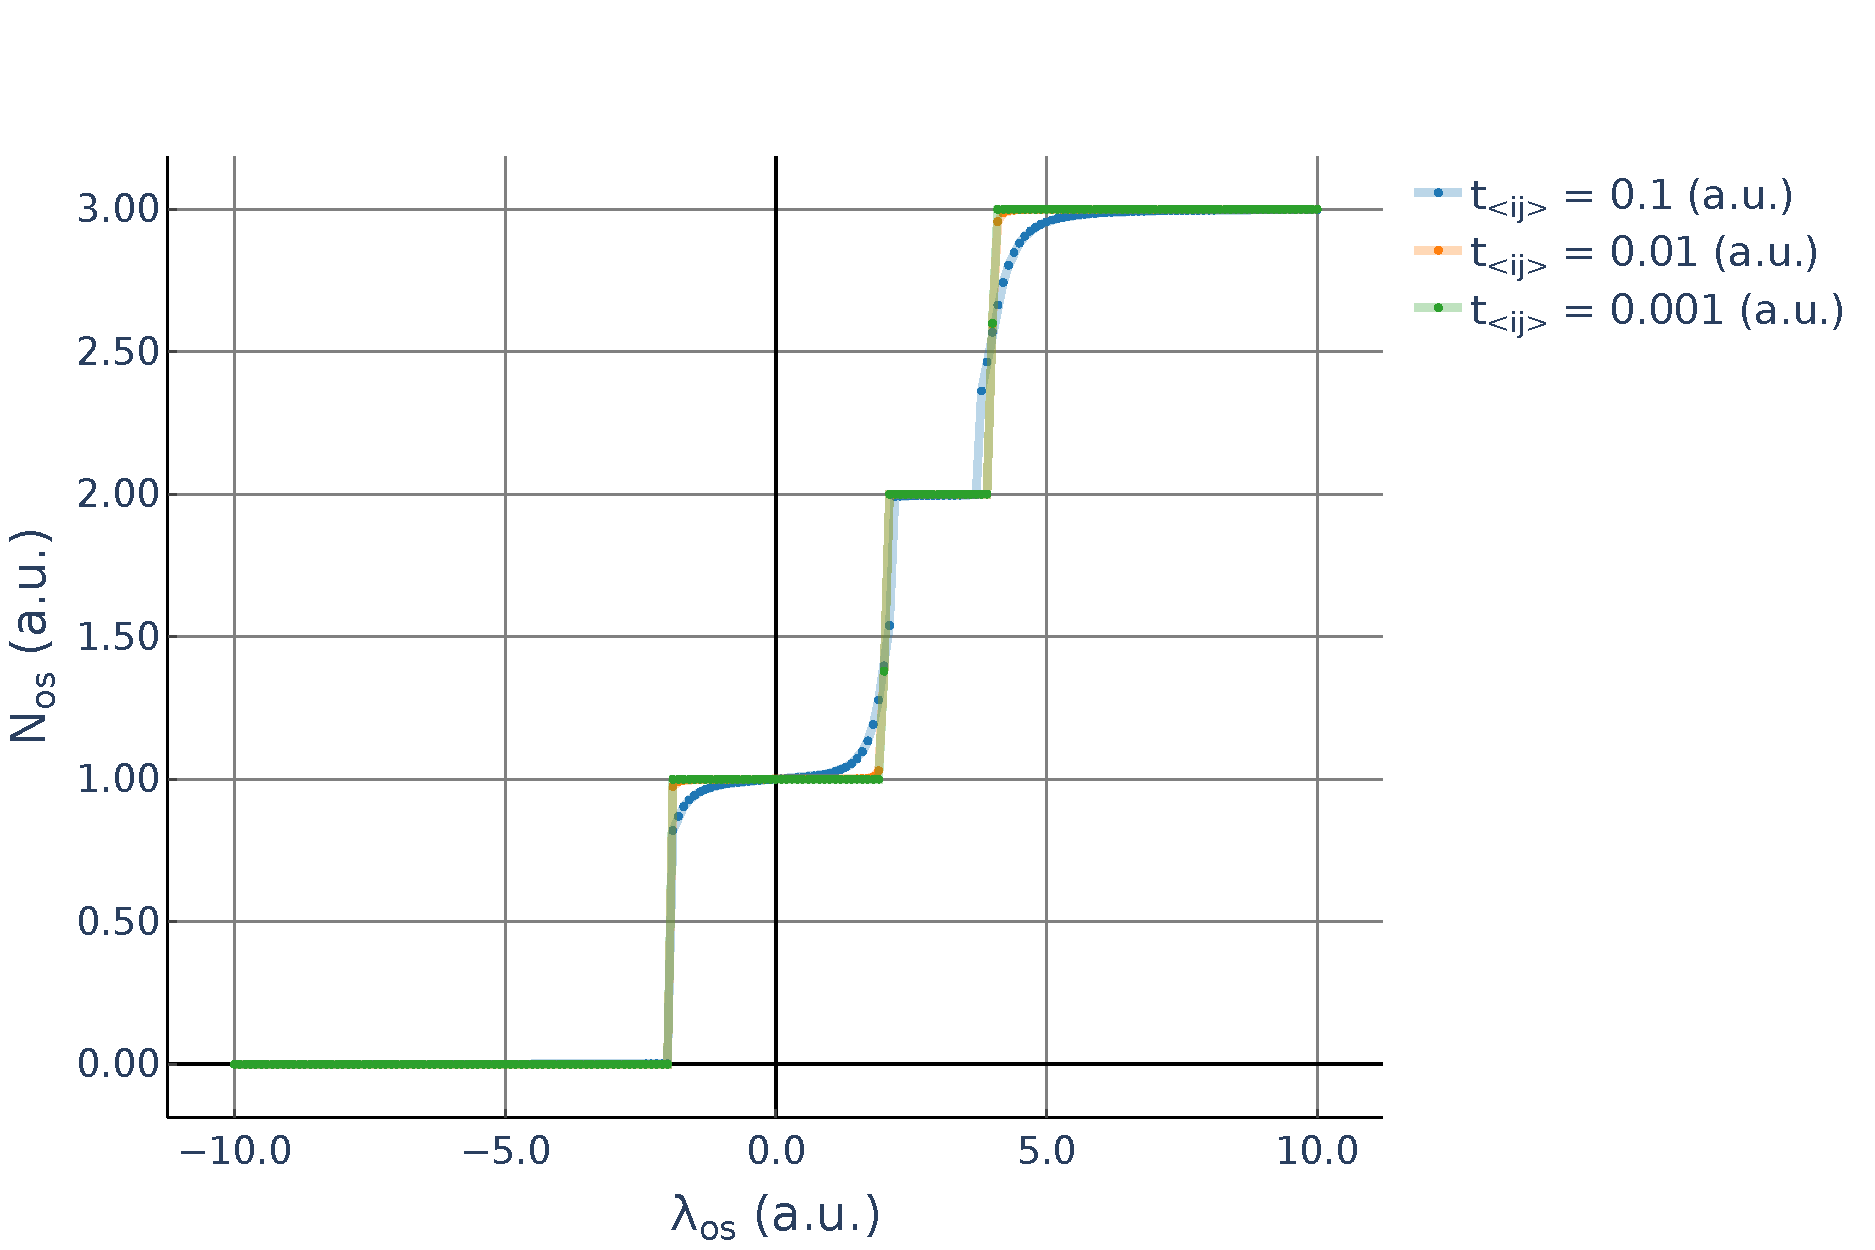
\includegraphics[width=\linewidth]{../code/figures/BH-3in3-NvsMu.pdf}
        \caption{Mott-Hubbard plateaus represented as the total open system population as a function of the applied chemical potential to the open subsystem for different values of $t_{ij}$.}
        \label{fig:Mott-Hubbard}
    \end{figure}
\end{center}
At high $U/t$, the Mott-plateaus restrict the movement of the bosons, indicating the system has transitioned to the MI-phase. The restriction of movement is also captured by the energy (\cref{fig:energetic-plateaus}), whose function becomes stepwise with energetic jumps occurring at the same critical $\lambda_{os}$ where the boson-exchange takes place.
\begin{center}
  \begin{figure}
      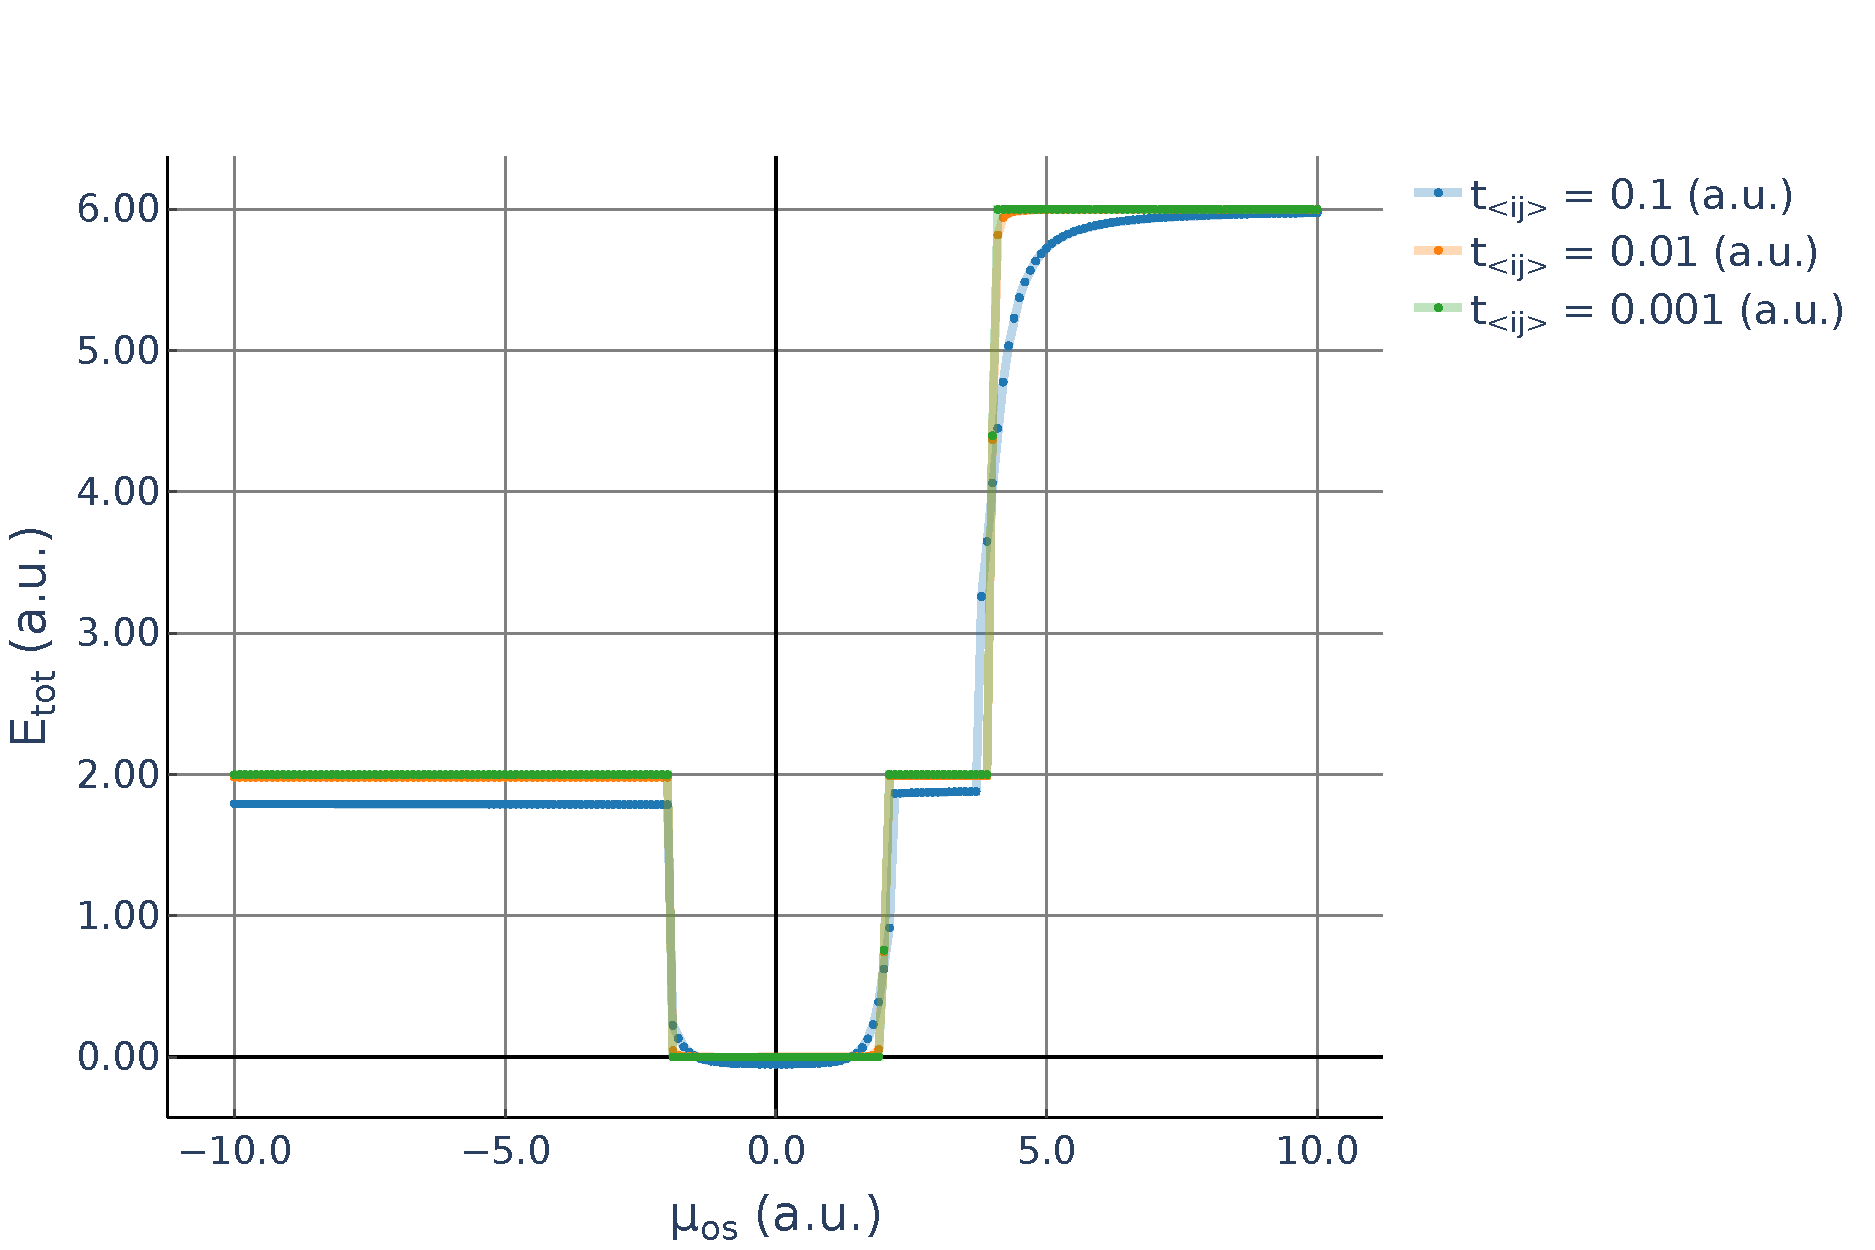
\includegraphics[width=\linewidth]{../code/figures/BH-3in3-EvsMu.pdf}
      \caption{Energetic Mott-Hubbard plateaus represented as a function of the applied chemical potential to the open subsystem for different values of $t_{ij}$.}
      \label{fig:energetic-plateaus}
  \end{figure}
\end{center}
The dual viewpoint which we can associate with these Mott-Hubbard plateaus is given by the energetic flat-planes \cite{perdew1982, cohen2008, cohen2012, yang2016}, where the total energy of the system ($E_{tot}$) becomes a series of straight line segments with discontinuities located at integer occupations (\cref{fig:flat-planes}). While previous results showed these characteristics for fermionic systems \cite{devriendt2021, devriendt2022}, we now show the same for the bosonic case.
\begin{center}
  \begin{figure}
      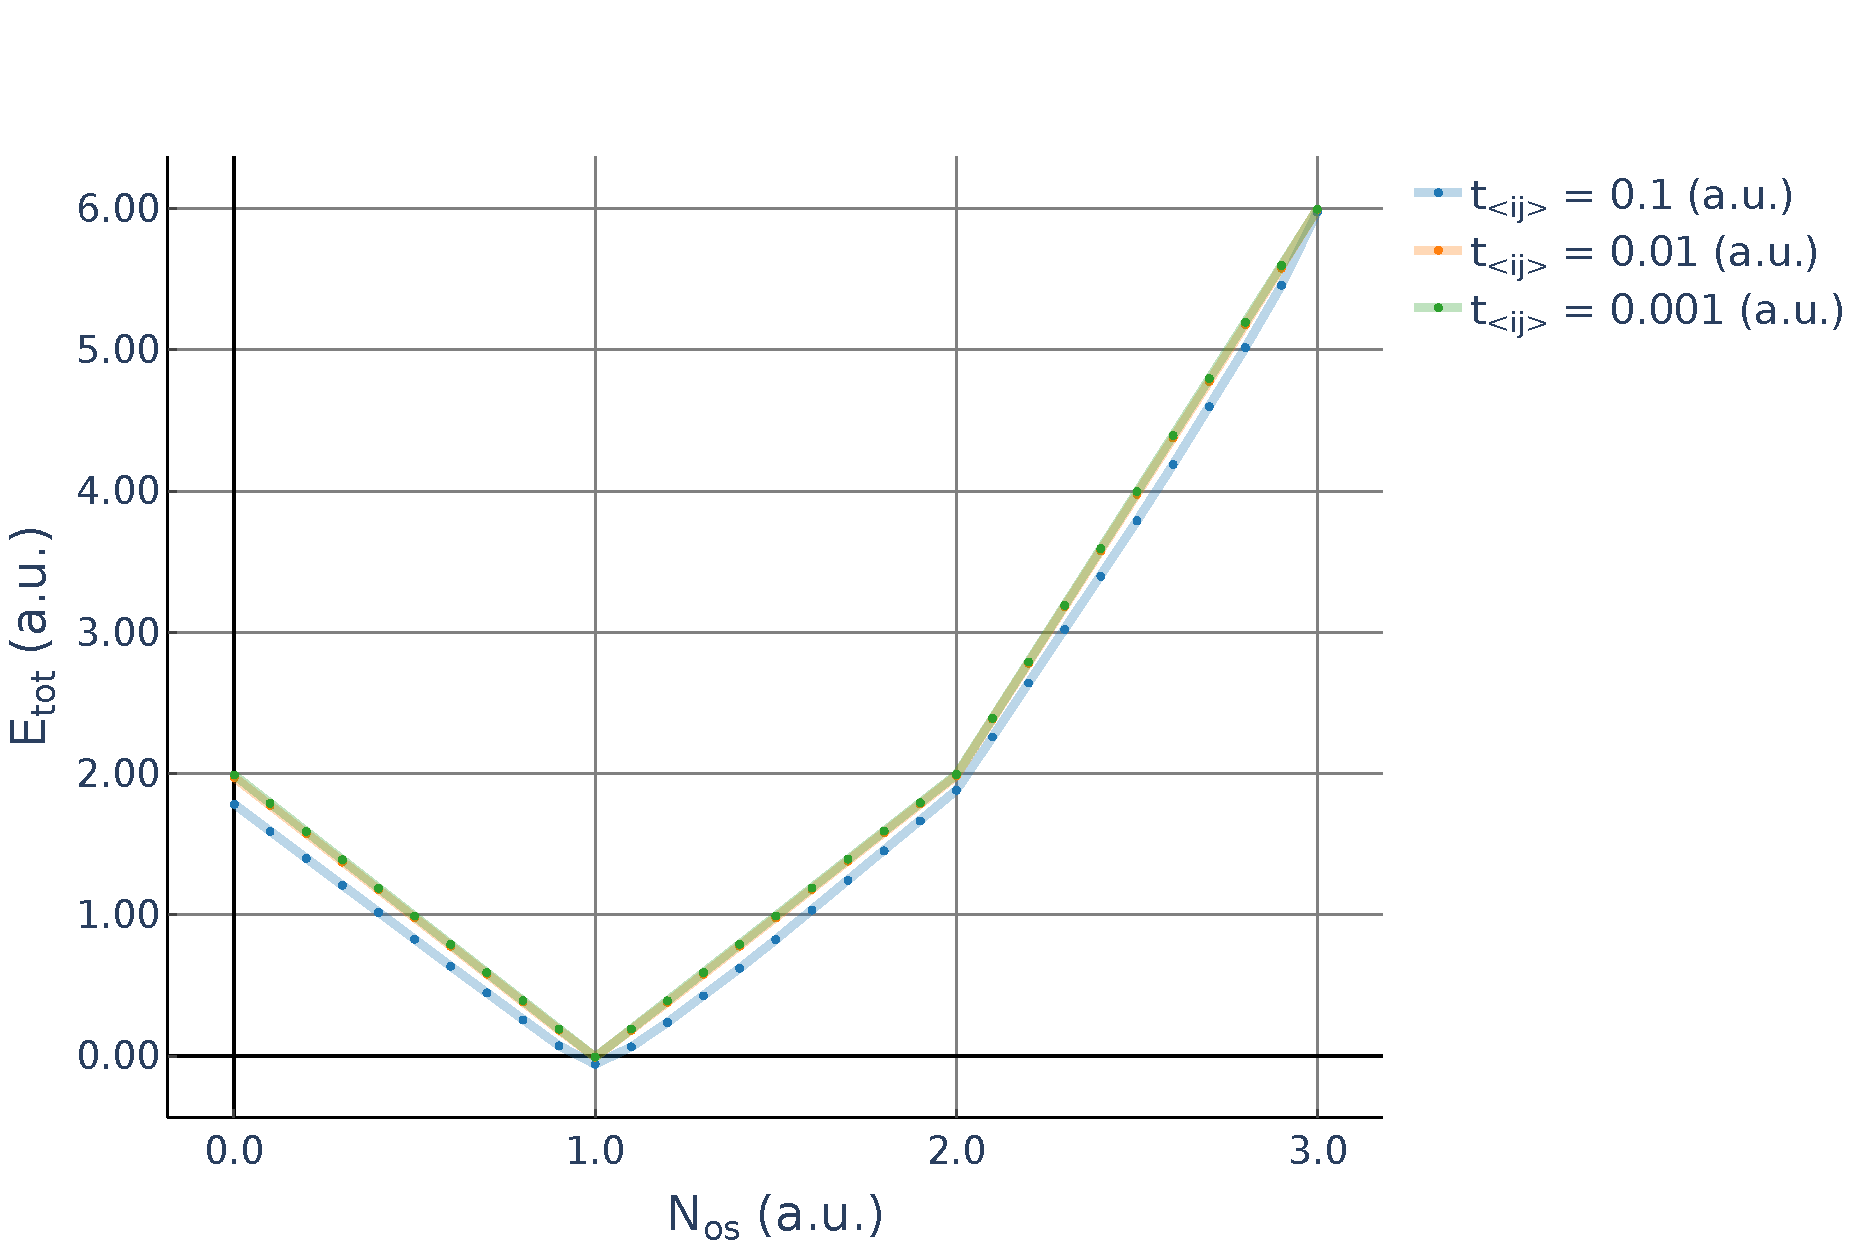
\includegraphics[width=\linewidth]{../code/figures/BH-3in3-EvsN.pdf}
      \caption{Energetic flat-planes represented by $E_{tot}$ as a function of the population of the open subsystem ($N_{os}$) for different values of $t_{ij}$.}
      \label{fig:flat-planes}
  \end{figure}
\end{center}

\subsection{DMRG can model the complete groundstate Bose-Hubbard phase diagram}

Instead of characterizing phase transitions based on population distributions in arbitrarily defined subsystems, it is also possible to model the phase diagram of the complete system. At integer filling of the sites ($\rho=\frac{N}{L}$) the one-dimensional Bose-Hubbard model describes a Mott transition (\cref{fig:Mott-Lobes}) between a so-called superfluid phase which is defined by a divergence of the momentum distribution at momentum $k$ equal to zero, and an MI phase, characterized by a finite gap for single particle excitations, defined by the difference between the potentials for half band filling and one particle less than half band filling (\cref{eq:gap}). However, in a six-site system this phase transition is not correctly described. Due to large finite-size effects, the single-particle excitation gap never closes (\cref{fig:Mott-Lobes-ED}) and the system remains in a Mott-Insulator band.
\begin{center}
  \begin{figure}
      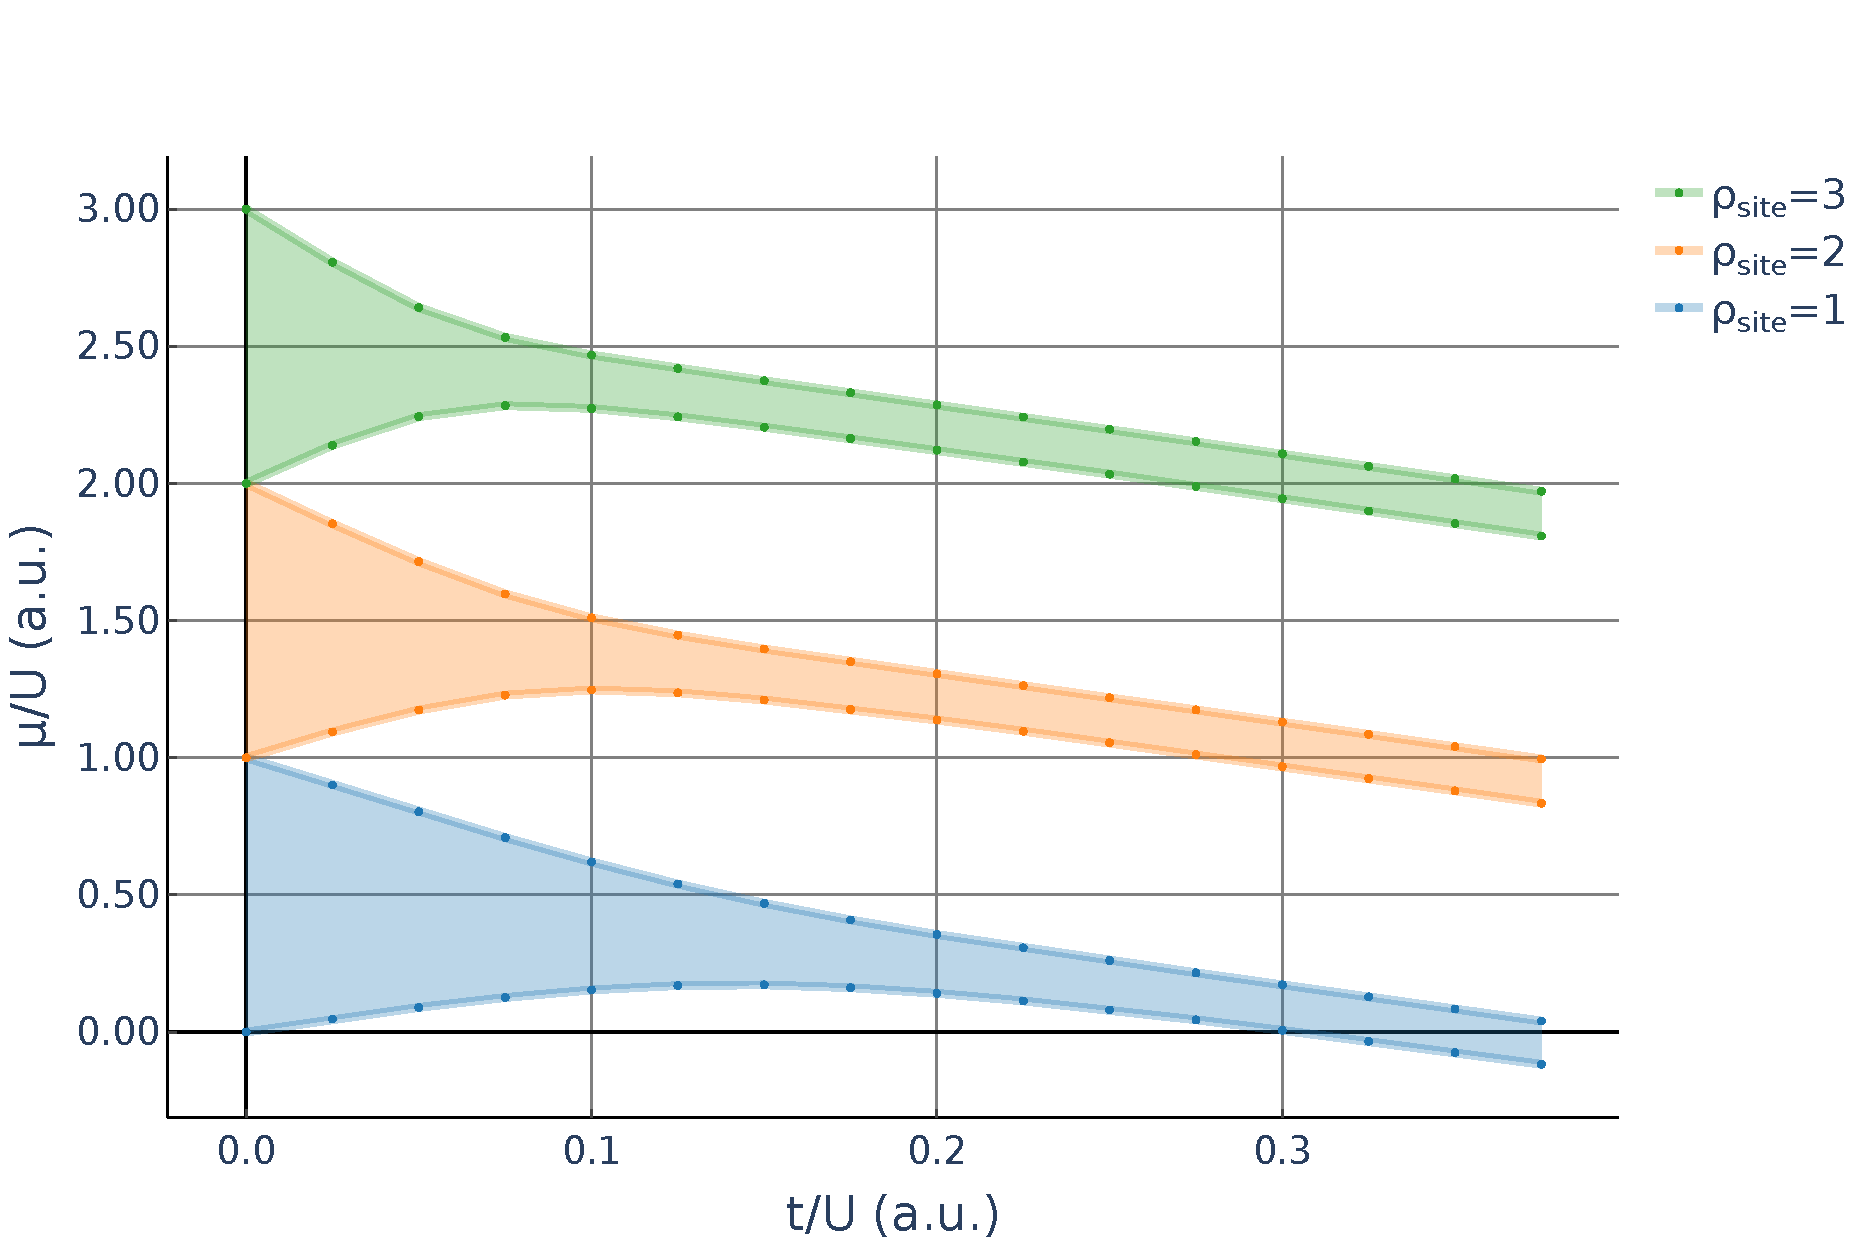
\includegraphics[width=\linewidth]{../code/figures/Mott-Lobes-ED.pdf}
      \caption{The first three Mott Lobes of the ground state Bose-Hubbard model. Colored sections represent the MI phases, while sections outside of the boundaries represent the superfluid phase. Calculated for $L=6$ with periodic boundary conditions using ED.}
      \label{fig:Mott-Lobes-ED}
  \end{figure}
\end{center}
Such small systems are incapable of providing information about the location of the critical point and the associated phase transition. To identify the critical point we enlarge the system to 128 sites. For such a system, DMRG is able to model the complete phase diagram (\cref{fig:Mott-Lobes}).
\begin{center}
  \begin{figure}
      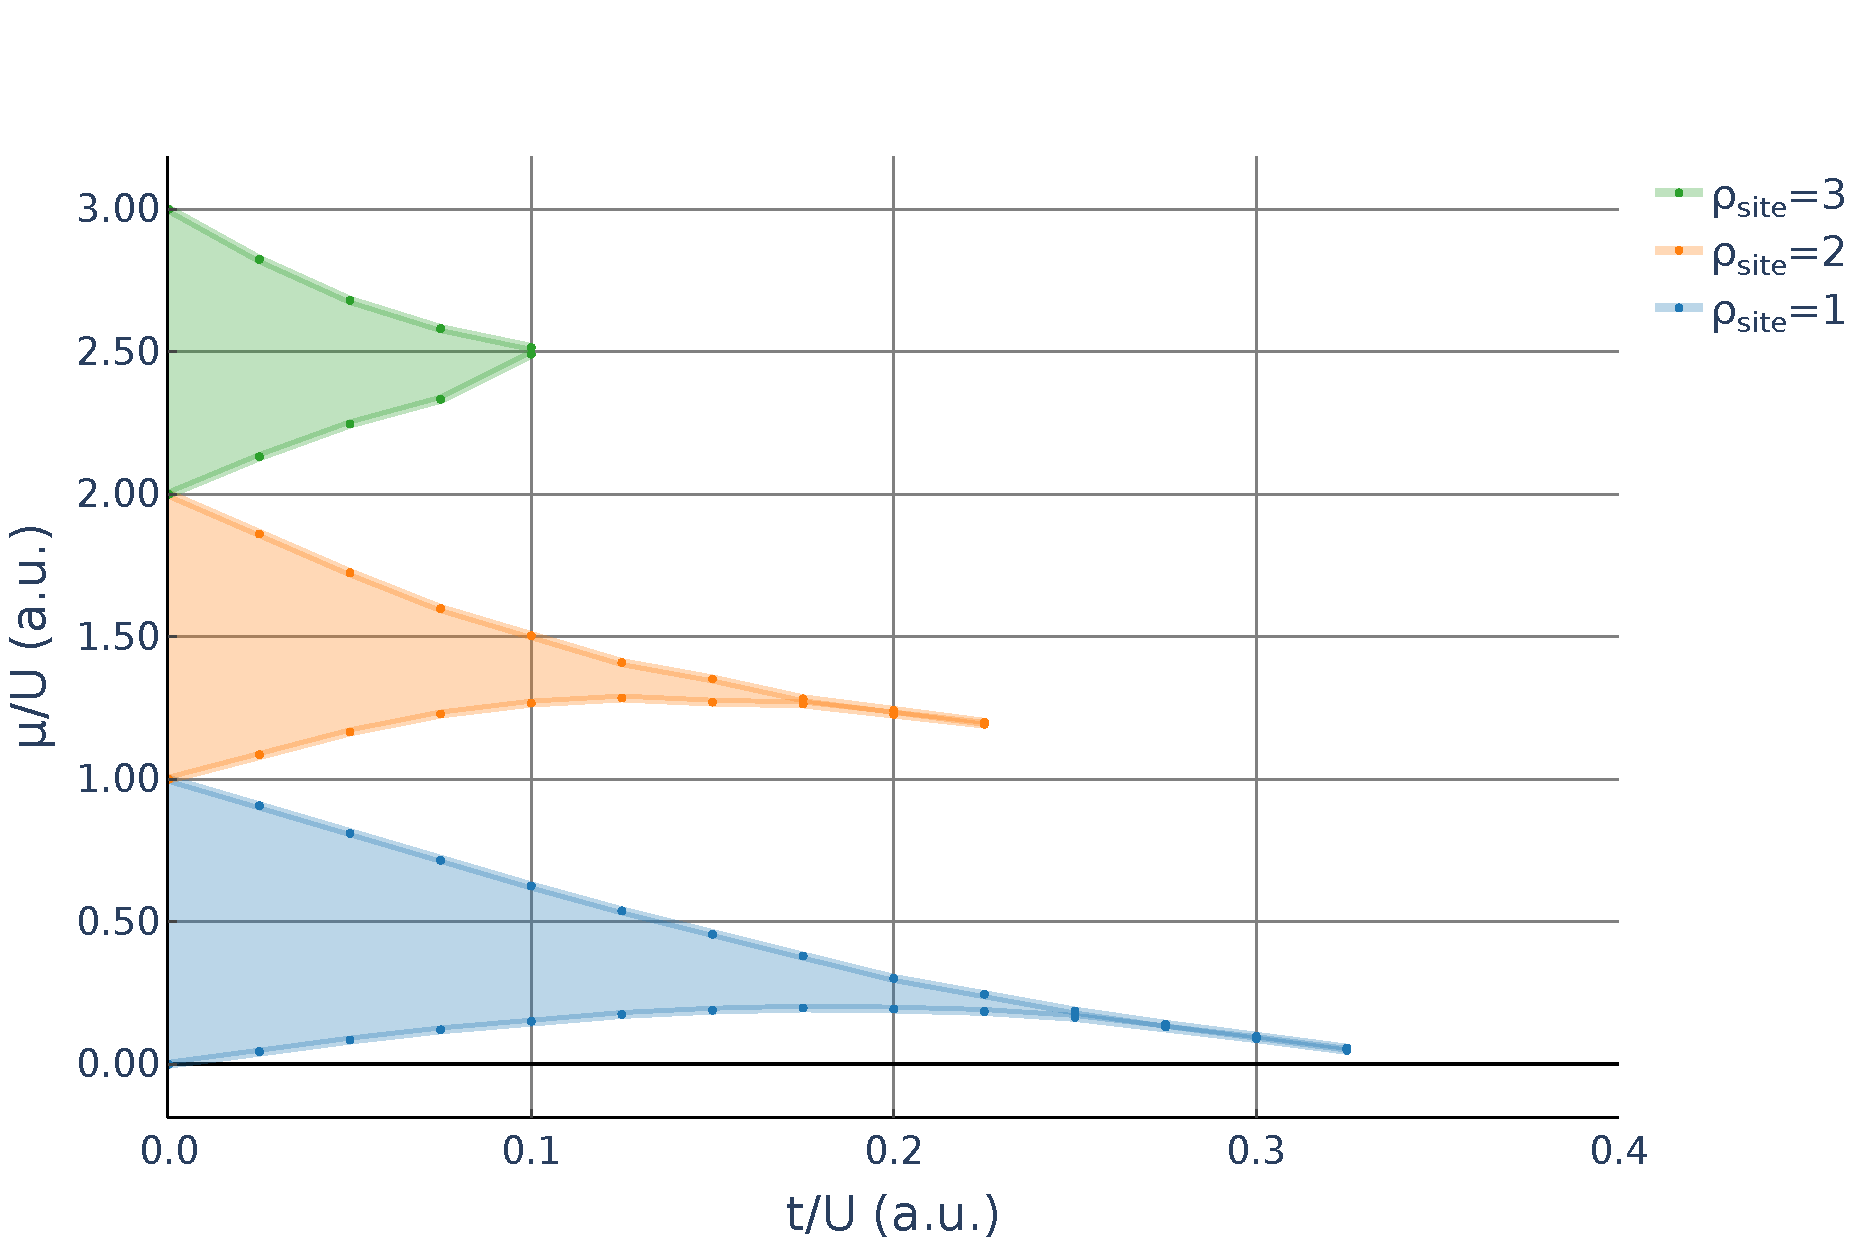
\includegraphics[width=\linewidth]{../code/figures/Mott-Lobes.pdf}
      \caption{The first three Mott Lobes of the ground state Bose-Hubbard model. Colored sections represent the MI phases, while sections outside of the boundaries represent the superfluid phase. Calculated for $L=128$ with open boundary conditions using the DMRG algorithm.}
      \label{fig:Mott-Lobes}
  \end{figure}
\end{center}
The single-particle excitation gap closes for every imposed integer density on the sites and several Mott lobes emerge, each with its own critical point. At the critical point, i.e. the tip of each Mott lobe, the model resides in the universality class of the XY-spin model, which indicates the presence of a BKT phase transition. In these Mott Lobes, the system has a constant, integer density on each site. Outside of the Mott-Lobes, the system enters a \emph{super critical state} in its particle number and no energy loss or gain is associated with changes in particle number.

\subsection{Superfluid Bose-Hubbard systems compensate impurities homogeneously across the system}

The bose-Hubbard model can be modified with the imposition of certain potentials ($\omega_i$, \cref{eq:bose-hubbard-hamiltonian}) on distinct sites of the lattice. Doing so disturbs to the otherwise uniform lattice and can be used to mimic impurities in solid state materials. Stabilizing impurities in the MI phase causes the bosonic population to increase on the affected sites, leading to compensation effects in the neighboring sites (\cref{fig:density-MI}), as the total particle number is preserved.
\begin{center}
  \begin{figure}
      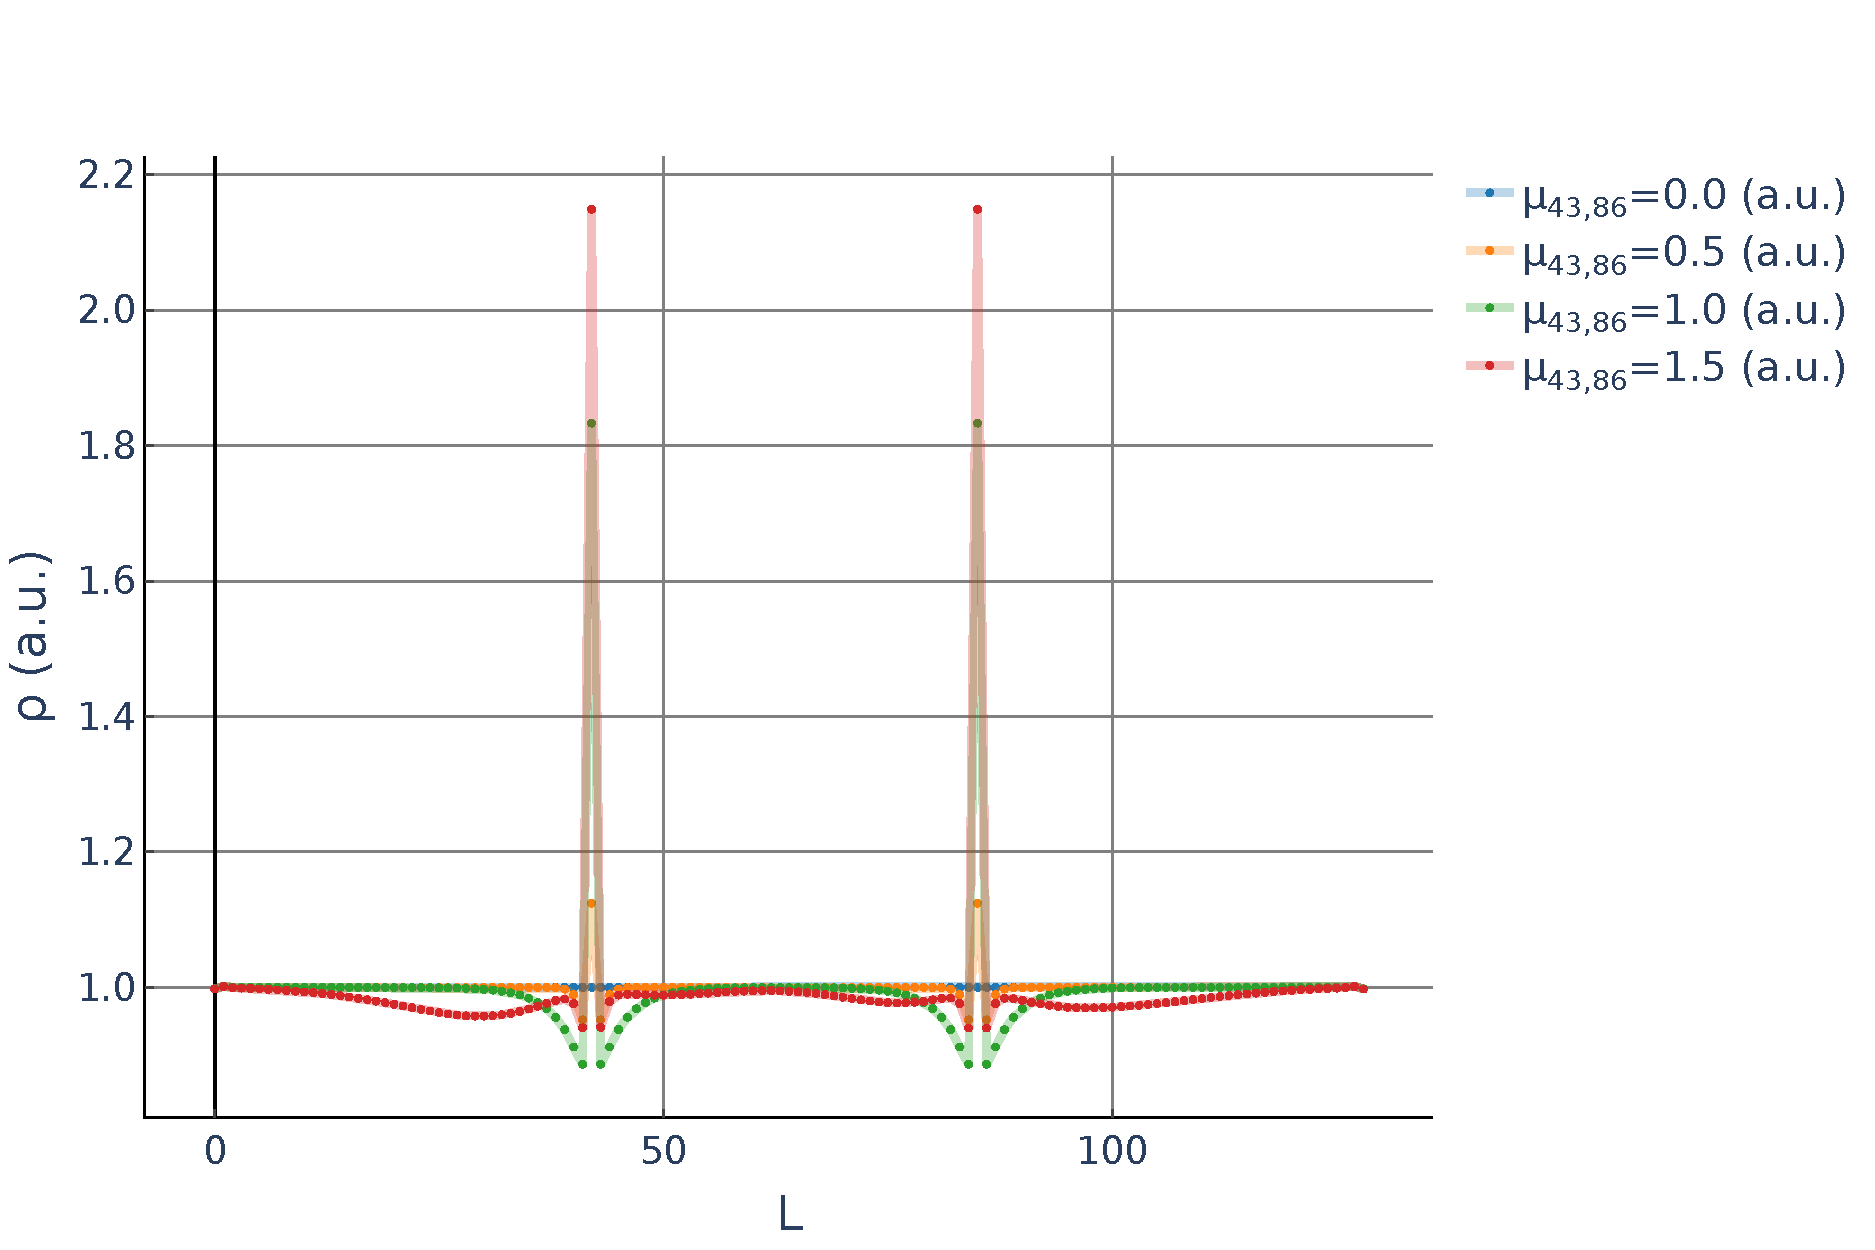
\includegraphics[width=\linewidth]{../code/figures/Density-profiles-MI.pdf}
      \caption{Density profile of a chain in the Mott-insulator phase containing 129 sites ($L$) and two impurities (site 43 and 86), with a stabilizing potential.}
      \label{fig:density-MI}
  \end{figure}
\end{center}
As the strength of the impurity increases, the the amount of sites needed to compensate for the impurity increases. The MI phase attempts to preserve the average density $\rho=1.0$ a.u. on as much of the lattice as possible. The SF phase on the other hand has no energetic advantage in preserving the average density on each site. Indeed, in order to adjust the system occupations with respect to the impurity, the average density on all sites gets shifted (\cref{fig:density-SF}) down.
\begin{center}
  \begin{figure}
      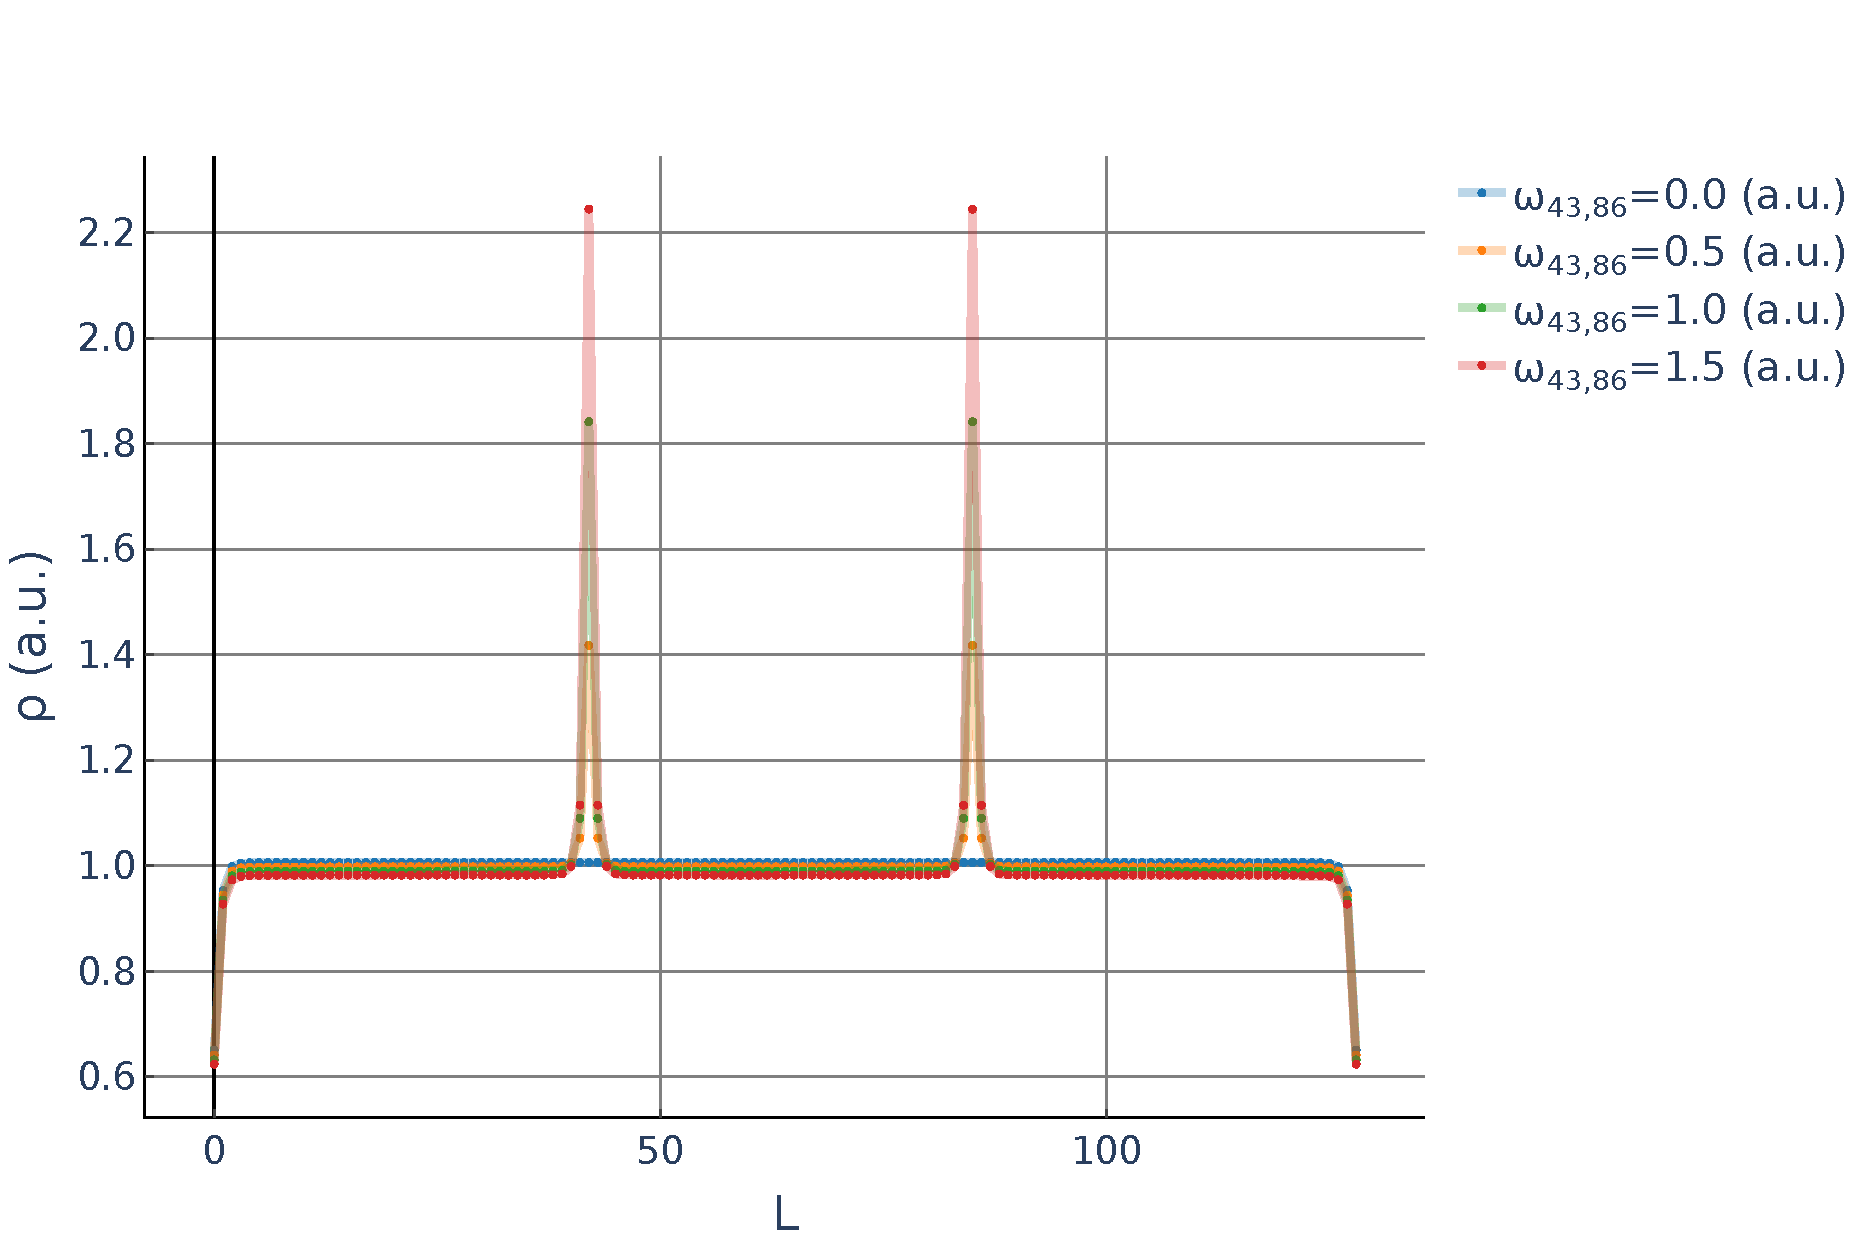
\includegraphics[width=\linewidth]{../code/figures/Density-profiles-SF.pdf}
      \caption{Density profile of a chain in the superfluid phase containing 129 sites ($L$) and two impurities (site 43 and 86), with a stabilizing potential.}
      \label{fig:density-SF}
  \end{figure}
\end{center}
The super-criticality in the particle number, associated with the SF phase, allows for the homogeneous compensation with respect to the impurities in the model.

\subsection{Fractional filling of the system induces density waves}

The system can also be brought in the superfluid phase at subcritical $U/t$ values by setting the total particle number in such a way that as an average, sites have a non-integer filling (\cref{eq:waves}). Such a fractional filling induces density waves throughout the system. These waves will have a frequency of $q$ sites for a fractional $\expval{\hat{n}} = \rho/q$ (\cref{fig:waves}). 
\begin{center}
  \begin{figure}
      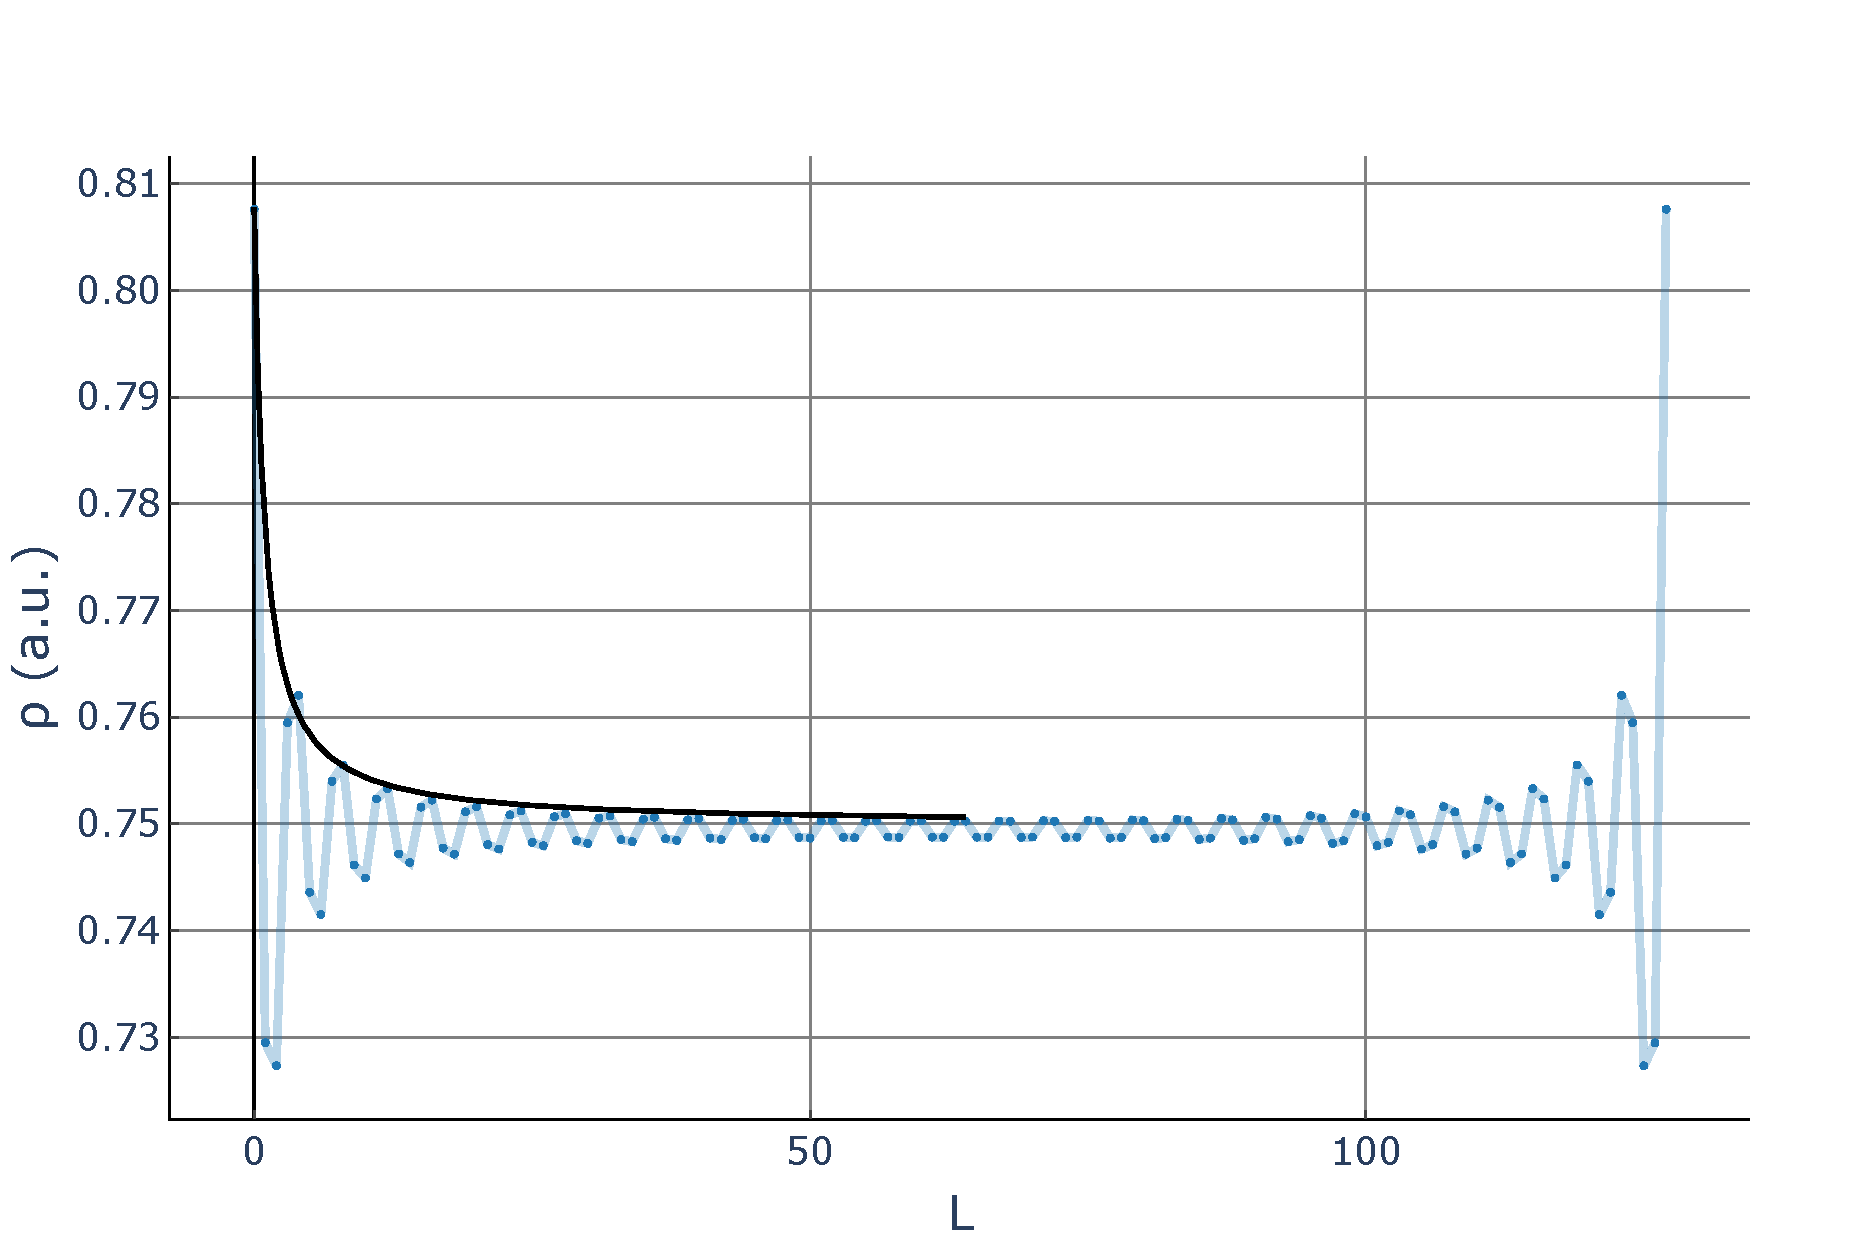
\includegraphics[width=\linewidth]{../code/figures/Density-profiles-fractional-density.pdf}
      \caption{Density profile of a chain in the superfluid phase containing 129 sites ($L$) with fractional filling $\rho=3/4$.}
      \label{fig:waves}
  \end{figure}
\end{center}
These density waves decay algebraically (see fit in \cref{fig:waves}) due to the edge effects present in the system with open boundary conditions. Introducing an impurity $\omega_i$ induces additional waves, whose wavelength  matches the inherent density waves of the system at the edges. However, their phase shifts depending on the impurity site  (\cref{fig:waves-impurity}). 
\begin{center}
  \begin{figure}
      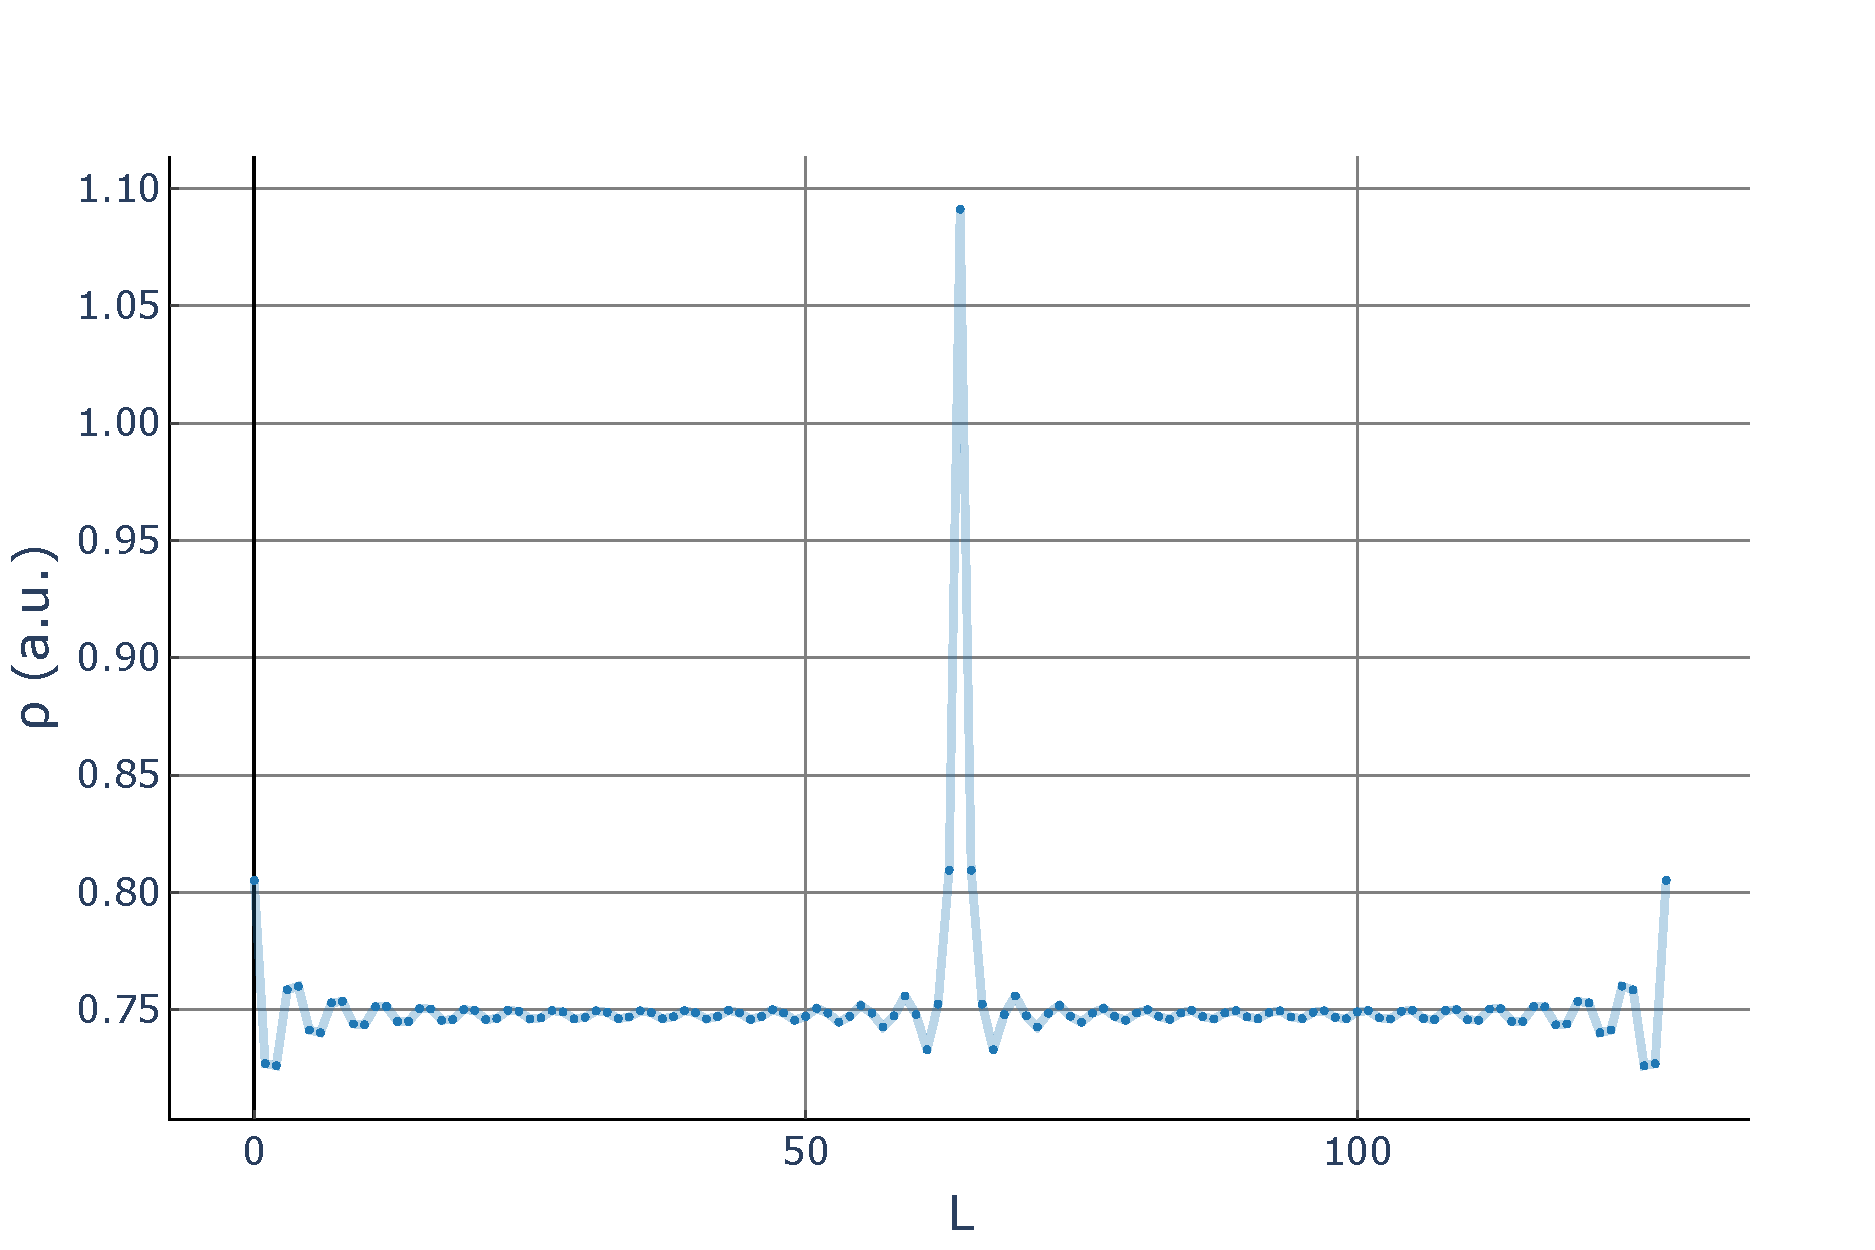
\includegraphics[width=\linewidth]{../code/figures/Density-profiles-fractional-impurity.pdf}
      \caption{Density profile of a chain in the superfluid phase containing 129 sites ($L$) with fractional filling $\rho=3/4$ and an impurity at site 65.}
      \label{fig:waves-impurity}
  \end{figure}
\end{center}
As such, complex interference effects are observed across the sites and cause the algebraic decay relation to fade. 

\subsection{Finite size effects and bond dimension influence the decay pattern of the correlation function}
One crucial difference between both phases of the Bose-Hubbard model is the manner in which the correlation function decays (\cref{eq:correlation decay}), i.e. exponentially in the MI phase and algebraically in the SF phase. Due to finite size effects and density waves introduced by the open boundary conditions the correlation function is calculated by averaging out the correlation between multiple site pairs with a distance $r$ in order to reduce their influence. 

In the MI phase, especially for small $t/U$, the correlation function decays exponentially with a small correlation length of only a few sites (\cref{fig:corMI1}). 
\begin{center}
  \begin{figure}
      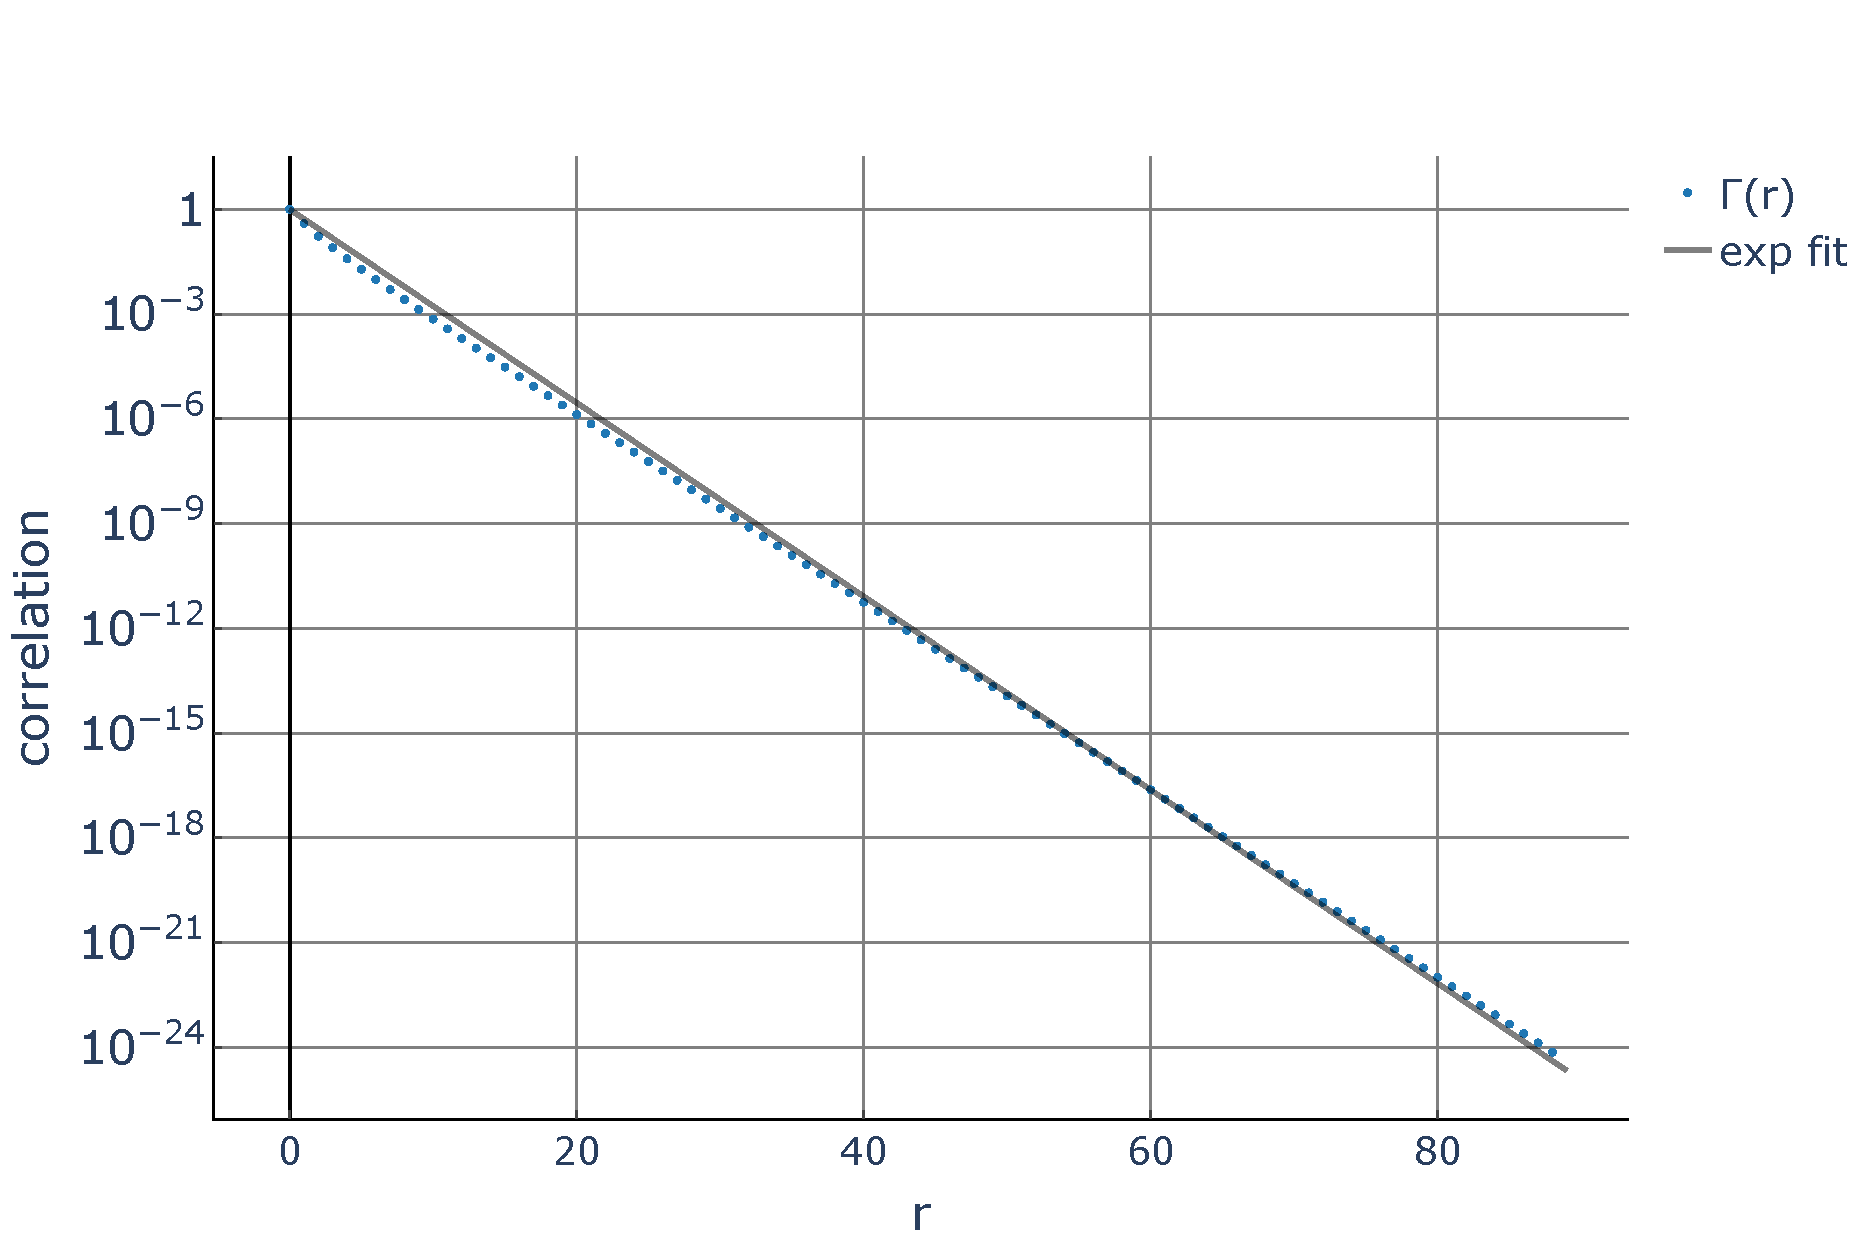
\includegraphics[width=\linewidth]{../code/figures/Correlations-MI1.pdf}
      \caption{Correlation function in the MI phase for a system with 128 sites for $t/U=0.1$ and $\rho=1$. Gray line represents an exponential fit. Y-axis is represented in log-scale.}
      \label{fig:corMI1}
  \end{figure}
\end{center}
Due to the fast decay, finite size effects and the effects of the density waves can almost be neglected. In the superfluid phase however, these effects cause the correlation to deviate from the expected fit (\cref{fig:corSF1}). As the distance starts to increase, the decay relation becomes algebraic.

The finite bond dimension used throughout the DMRG algorithm limits the correlation length, causing the decay of the correlation function to transition towards an exponential fit starting at approximately $r=50$.
\begin{center}
  \begin{figure}
      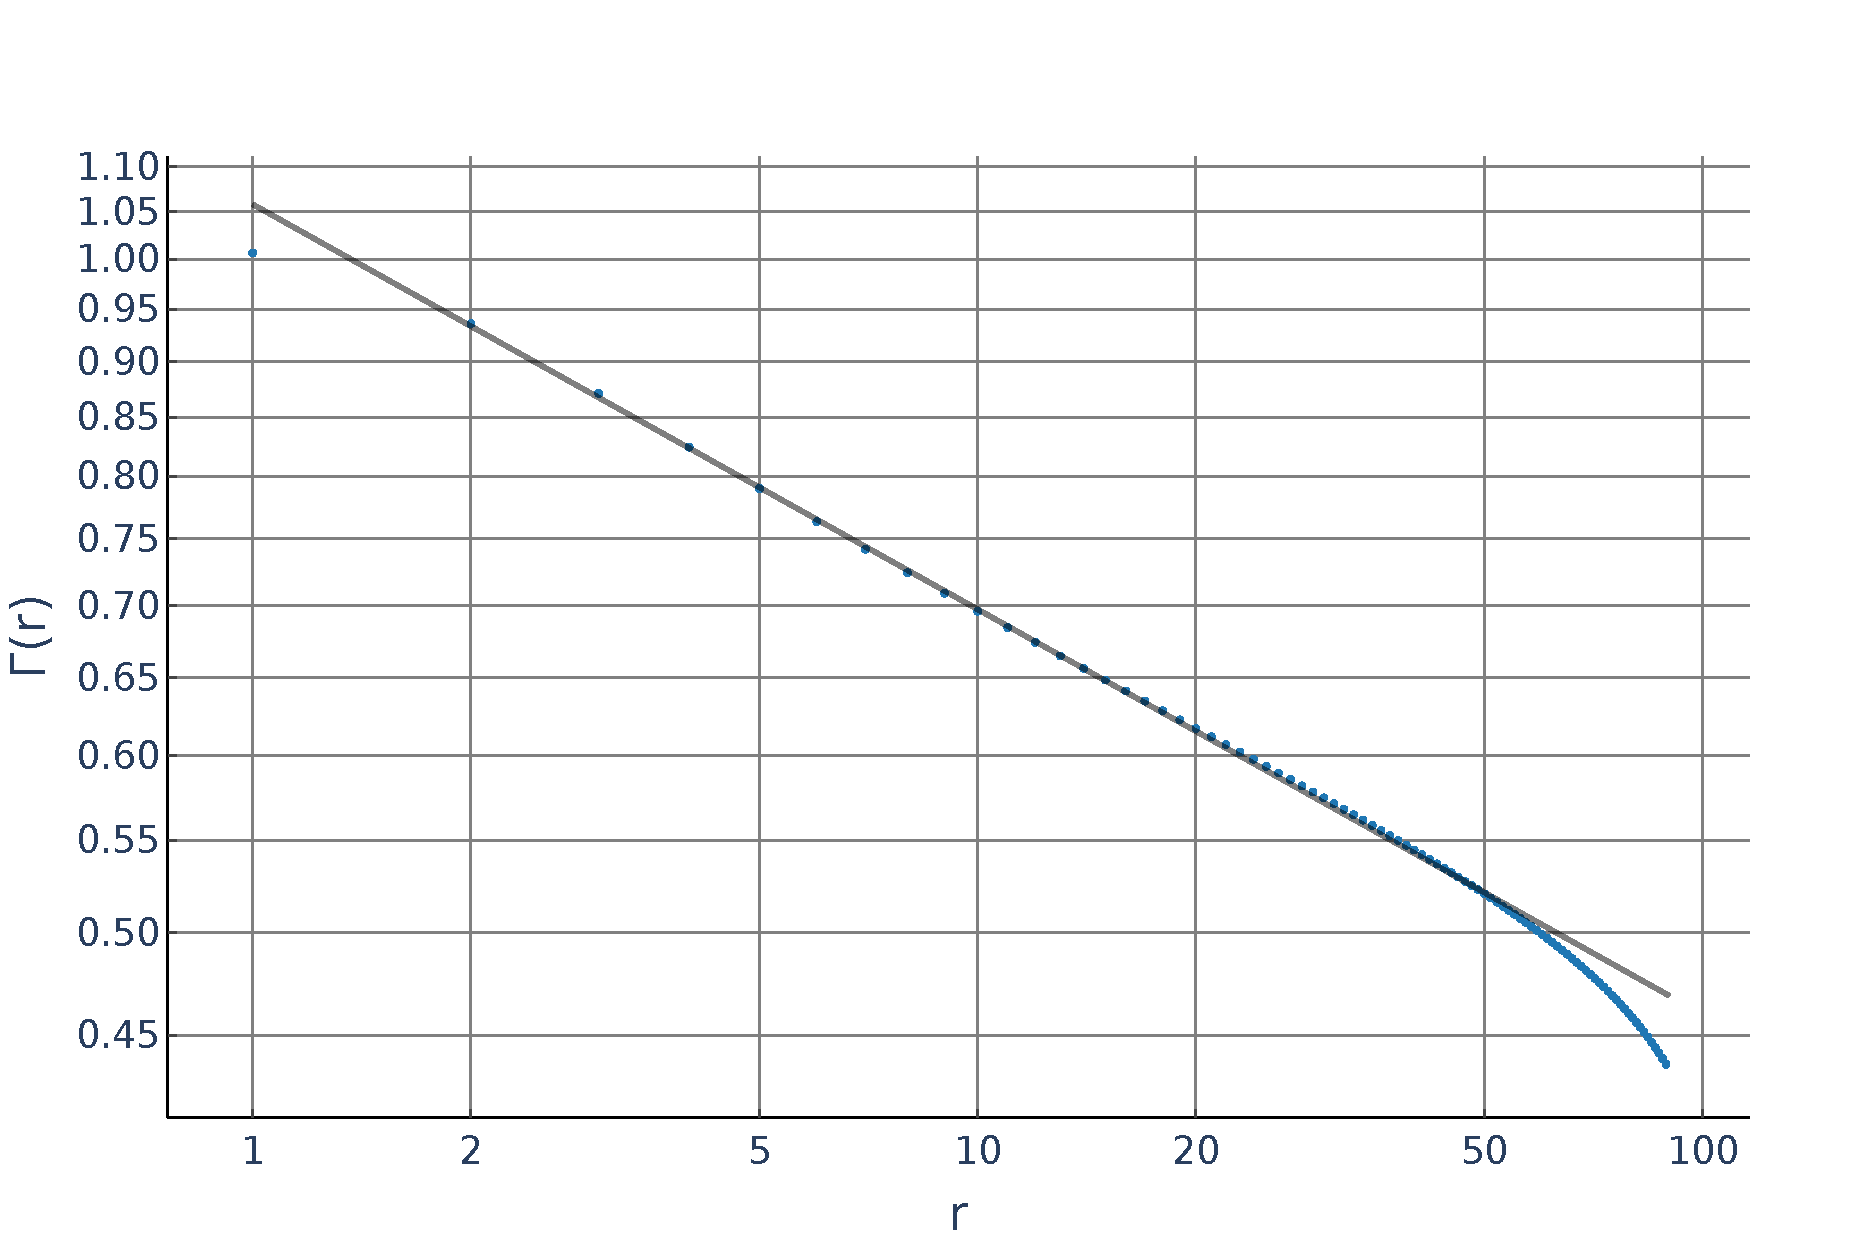
\includegraphics[width=\linewidth]{../code/figures/Correlations-SF1.pdf}
      \caption{Correlation function in the SF phase with 128 sites for $t/U=0.5$ and $\rho=1$. Gray line represents a power law fit. Both axes are represented in log-scale.}
      \label{fig:corSF1}
  \end{figure}
\end{center}
When inducing the transition to the superfluid phase by imposing a fractional average occupation per site, at sub-critical $t/U$ values, the decay is qualitatively identical to the large $t/U$ case, but occurs much slower (\cref{fig:corSF2}).
\begin{center}
  \begin{figure}
      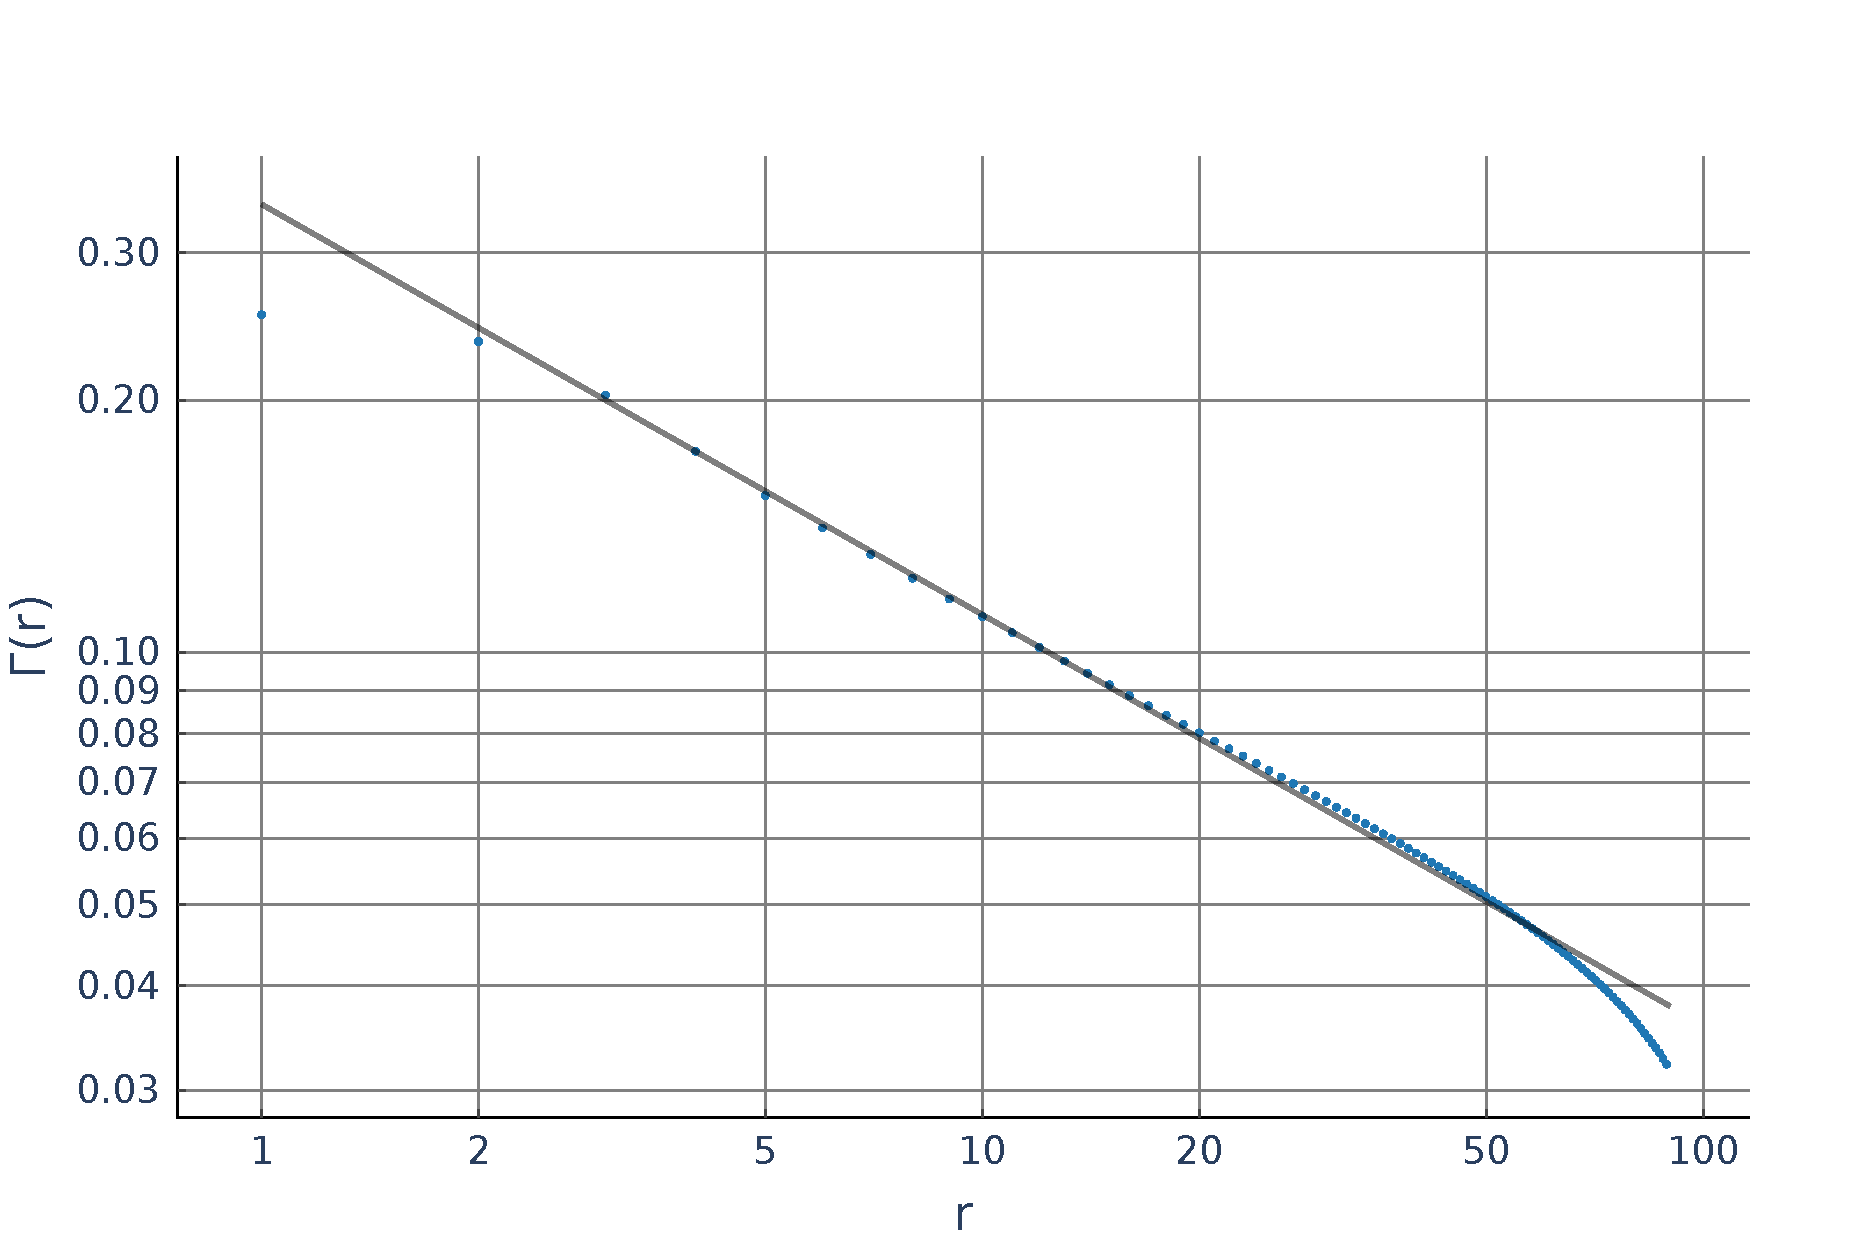
\includegraphics[width=\linewidth]{../code/figures/Correlations-SF2.pdf}
      \caption{Correlation function in the SF phase with 128 sites for $t/U=0.1$ and $\rho=1/4$. Gray line represents a power law fit. Both axes are represented in log-scale.}
      \label{fig:corSF2}
  \end{figure}
\end{center}
 
By calculating the correlation function for increasing values of maximum bond dimension $D$ we are able to accurately quantify the resulting errors caused by these finite size effects. Once $D$ transcends past $D=64$ there is no longer any notable difference in the induced errors (\cref{fig:bonds}). 
\begin{center}
  \begin{figure}
      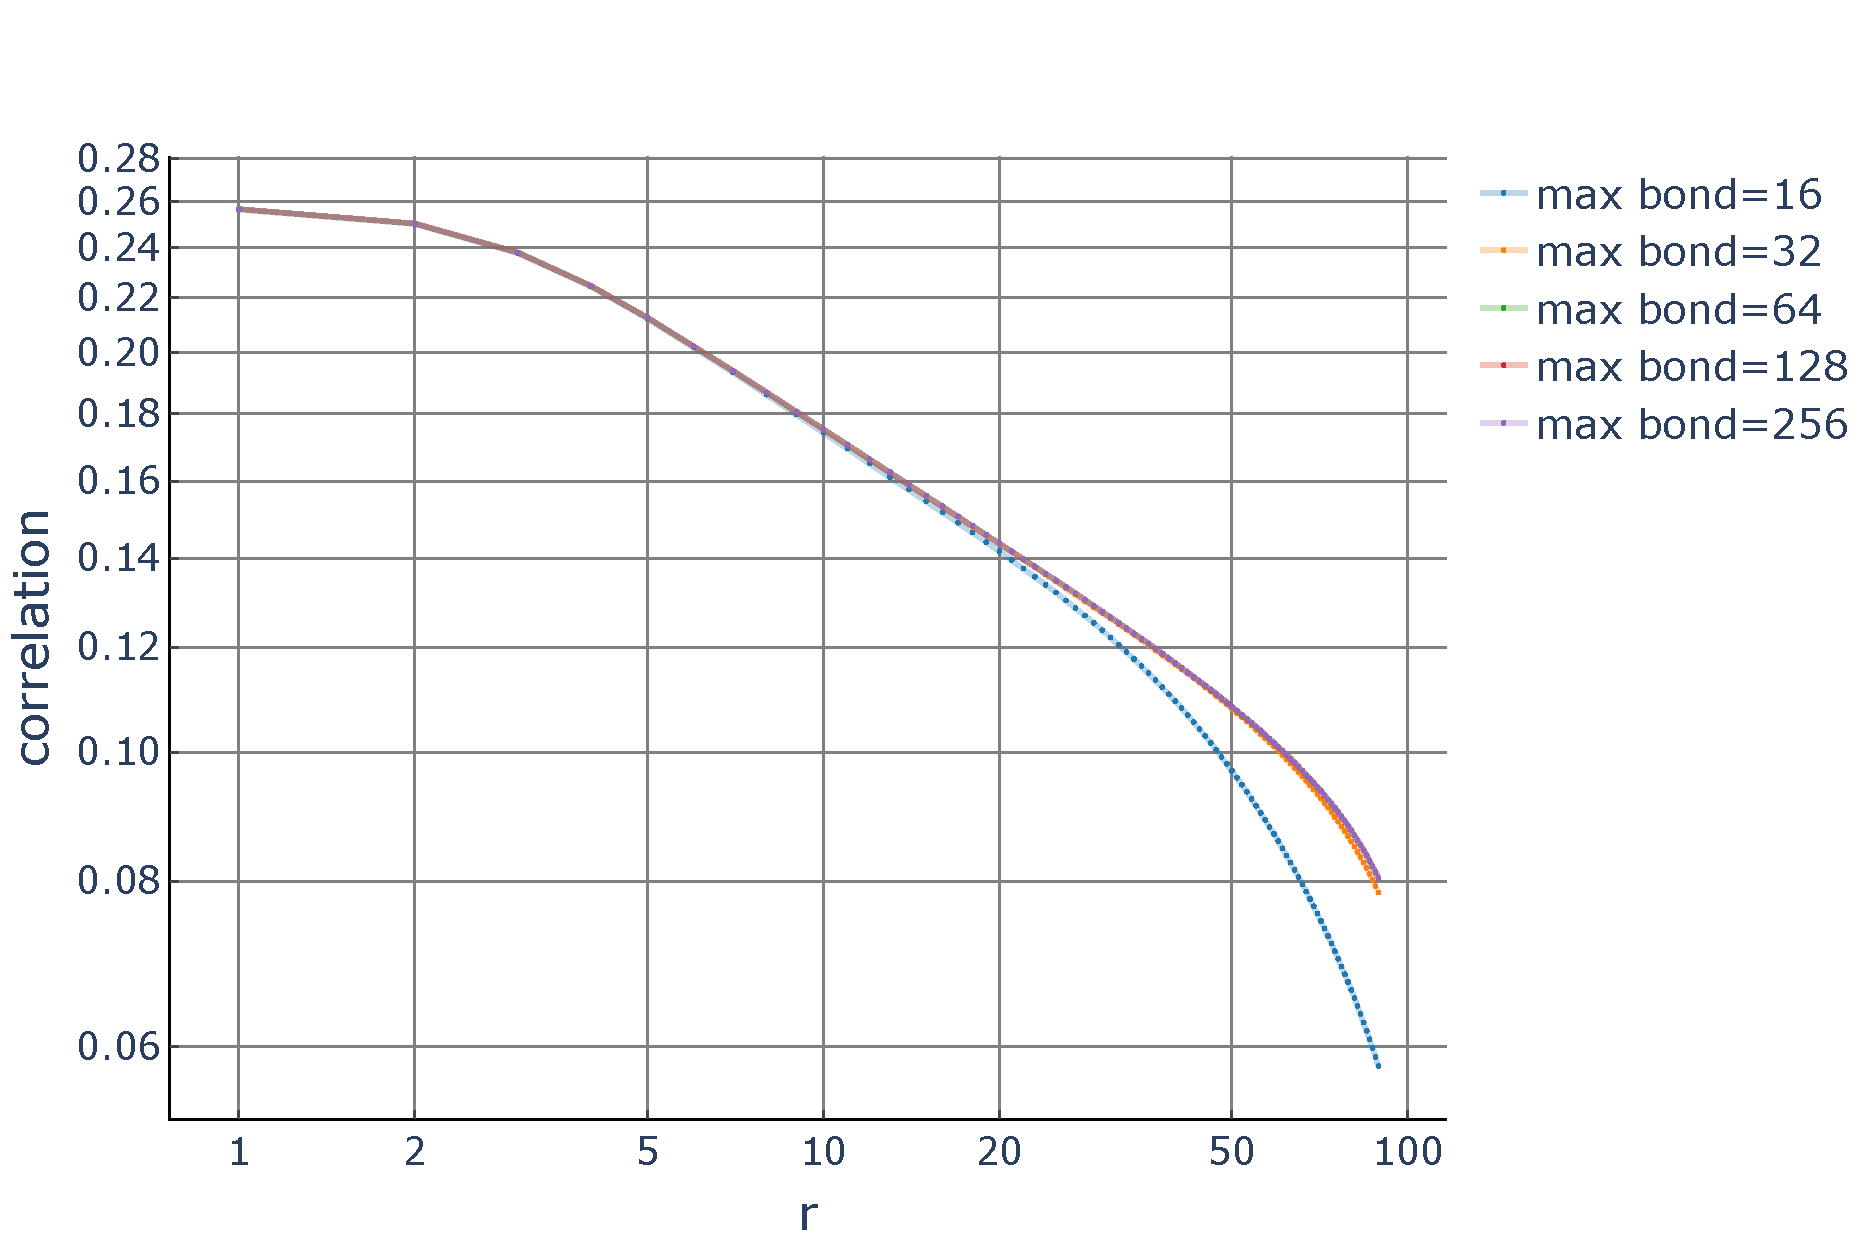
\includegraphics[width=\linewidth]{../code/figures/Correlations-bonds.pdf}
      \caption{Correlation functions in the SF phase with 128 sites and different maximum bond dimensions ($D$). Both axes are represented in log scale.}
      \label{fig:bonds}
  \end{figure}
\end{center}
However, at large $r$ values, the decay still becomes exponential, even at $D\ge64$. Calculations for different system sizes at a constant $D$ elucidate that the decay functions still decay exponentially at large $r$ values (\cref{fig:lengths}). As such, decay function becoming exponential has its root in the systematic errors due to finite size. The initial algebraic decay remains indifferent with respect to system size and is sufficiently well documented starting at $L=128$.
\begin{center}
  \begin{figure}
      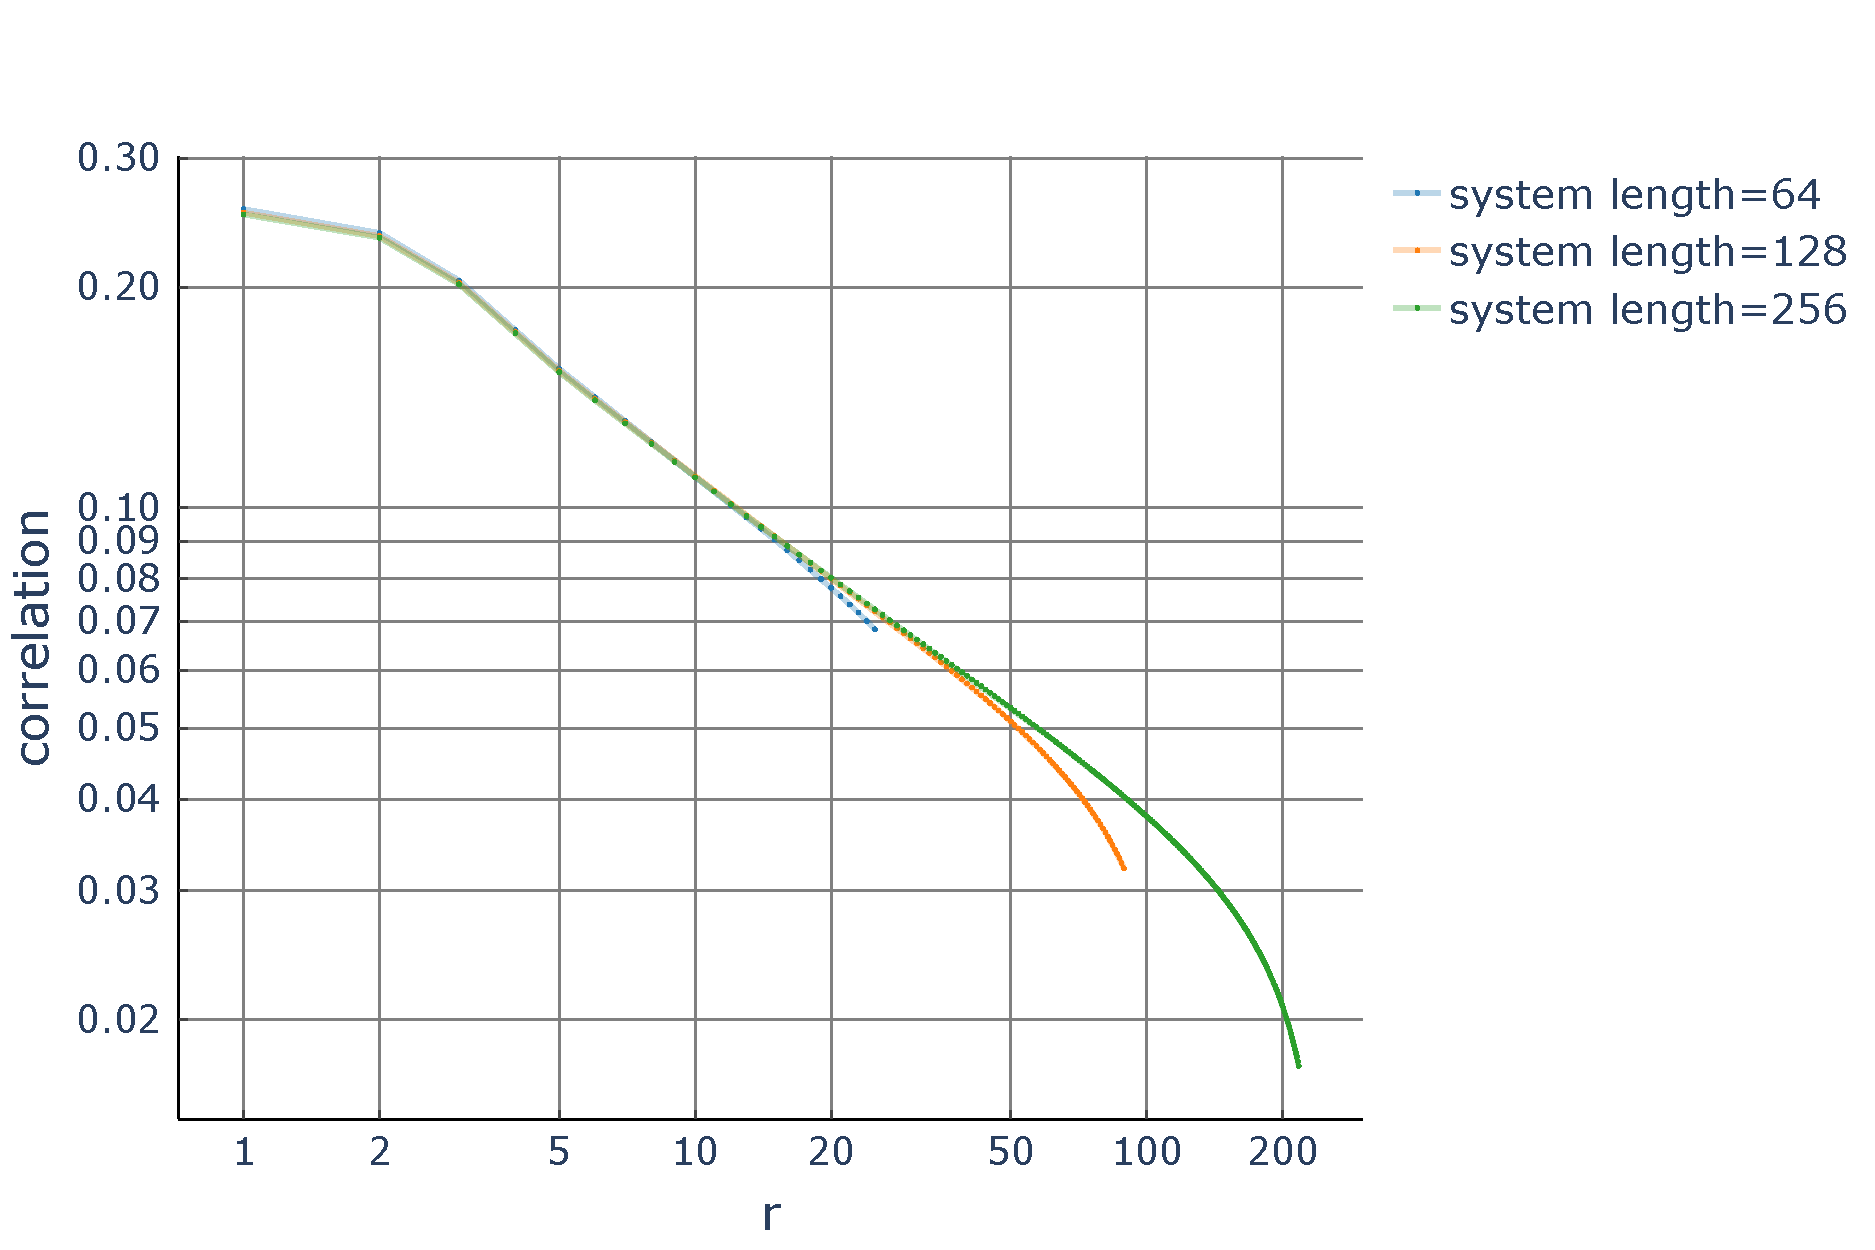
\includegraphics[width=\linewidth]{../code/figures/Correlations-lengths.pdf}
      \caption{Correlation functions in the SF phase with for different sizes of finite chains, with constant bond dimension. Both axes are represented in log scale.}
      \label{fig:lengths}
  \end{figure}
\end{center}

\subsection{Correlation function and its decay indicate the presence of the critical point $t_c$}

Modelling the critical point $t_c$ of a BKT-transition is very computationally demanding due to the fact that the correlation length diverges non-perturbatively making small errors due to finite size and bond dimension cause large differences in calculated values. In the MI phase however, its presence can still be seen by the rapidly increasing correlation length towards $t/U\approx 0.3$ (\cref{fig:cor lengths}), modelled by fitting an exponential function to the correlation function at different values of $t$. 
\begin{center}
  \begin{figure}
      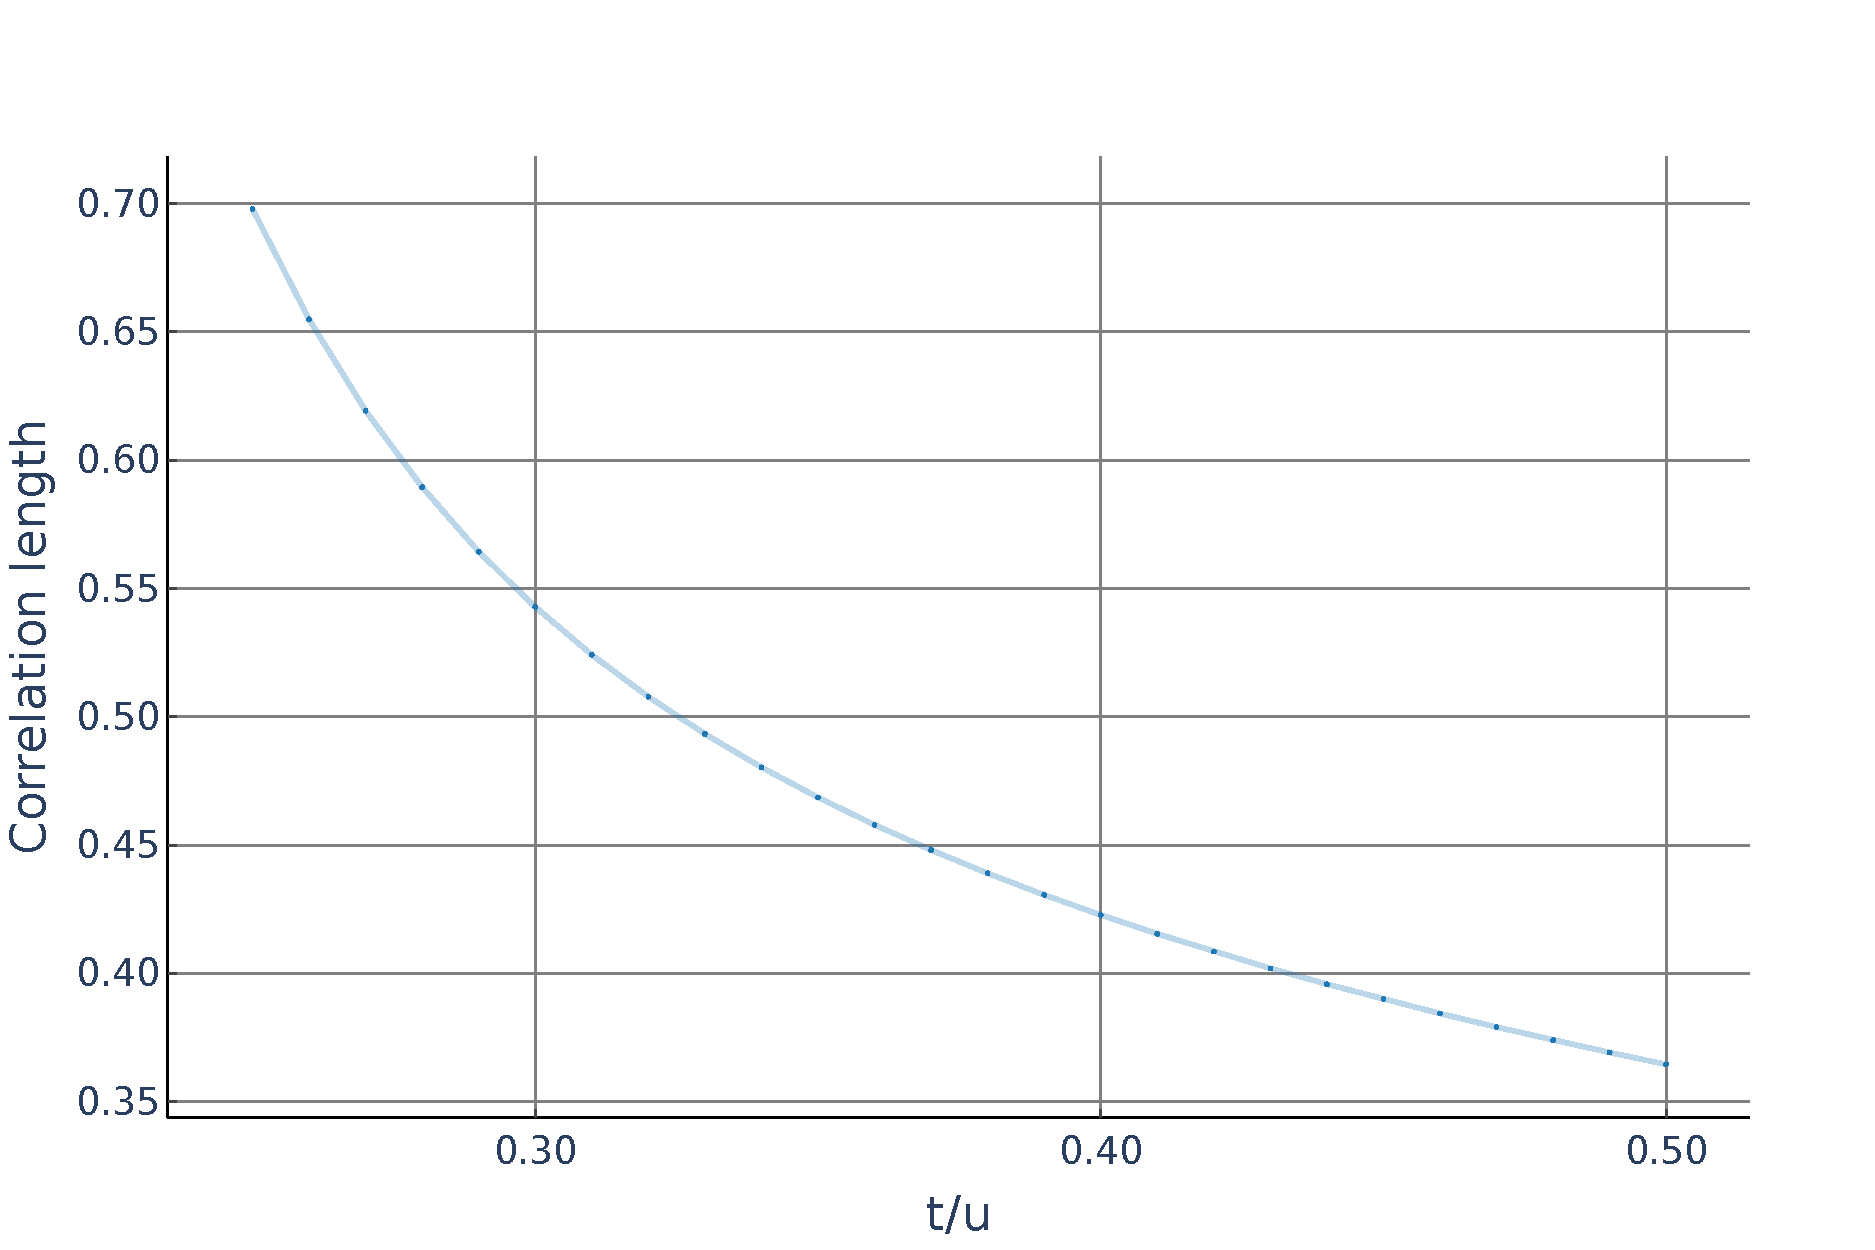
\includegraphics[width=\linewidth]{../code/figures/Correlations-length-values.pdf}
      \caption{Correlation lengths in the MI phase for different values of $t/U$ and $\rho=1$. Calculated for a system with $L=128$ and open boundary conditions.}
      \label{fig:cor lengths}
  \end{figure}
\end{center}
Finite size effects and finite bond dimension still prevent the correlation length from diverging, however. 

In the superfluid phase, the critical value of $K$ (\cref{eq:power decay}), i.e. $K_c$ can be approximated by fitting a power law to the algebraically decaying correlations (evidenced by \cref{fig:corSF1}, \cref{fig:corSF2}, \cref{fig:bonds} and \cref{fig:lengths}). To circumvent the fact that the algebraic decay relation only applies for non-integer average occupations at small $t/U$, the correlation functions are calculated for $\rho\rightarrow n$ with $n$ an integer value. When the average density on each site equals one ($n=1$), the critical $K_c$ can be calculated to be $K_c=1/2$ (using \cref{eq:Kc}). By approximating the density in $\rho\rightarrow n$ as $\rho=31/32$, the critical value found is approximately $K_c\approx 0.33$ (\cref{fig:K values}).
\begin{center}
  \begin{figure}
      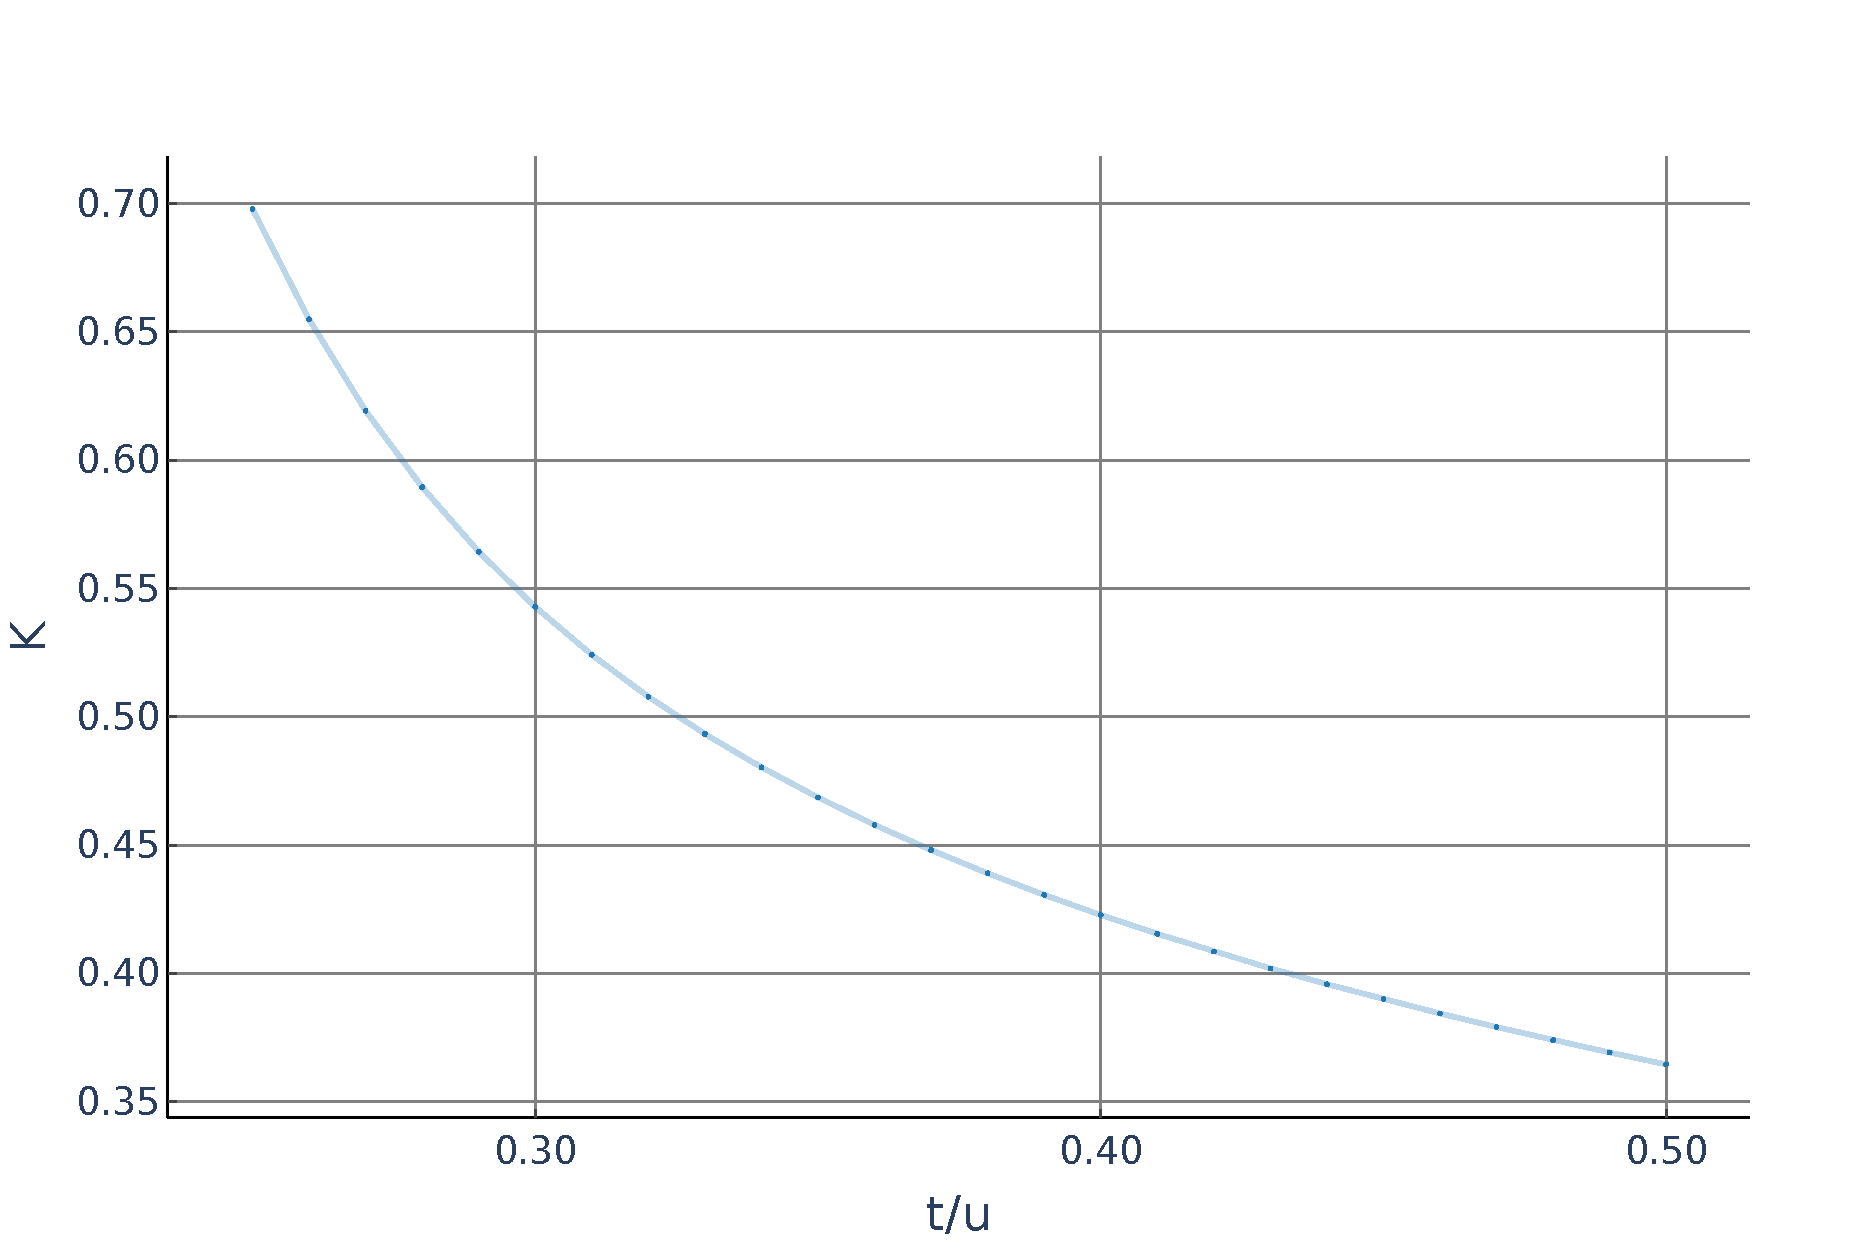
\includegraphics[width=\linewidth]{../code/figures/Correlations-K-values.pdf}
      \caption{Correlation lengths in the SF phase for different values of $t/U$ and $\rho=31/32$.}
      \label{fig:K values}
  \end{figure}
\end{center}
This result is too high, presumably because the density does not approach $n=1$ closely enough.

\section{Conclusions}

In this study we showed that occupation redistributions with exact diagonalization techniques give an indication about the possible phase transitions of the system. However, due to the limitations of these techniques, MPS methods and the DMRG algorithm are required to model the complete phase diagram. Using this phase diagram, we have shown how the different phases deal with the introduction of impurities to the lattice and that the contribution of finite size effects contributes more to the systematic errors than a finite bond dimension. Finally, we have proven that the methodology used can already give a good indication of the critical point if the systematic errors of the algorithm are properly taken into account, even though the critical point of a BKT transition is notoriously difficult to describe.

% \section*{Acknowledgements}

% \begin{itemize}
%   \item FWO, BOF 
%   \item HPC 
% \end{itemize}

%%%END OF MAIN TEXT%%%

%The \balance command can be used to balance the columns on the final page if desired. It should be placed anywhere within the first column of the last page.

%\balance

%If notes are included in your references you can change the title from 'References' to 'Notes and references' using the following command:
%\renewcommand\refname{Notes and references}
%%%REFERENCES%%%
\bibliography{outline} %You need to replace "rsc" on this line with the name of your .bib file
\bibliographystyle{aip} %the AIP's .bst file

\end{document}
